\documentclass[12pt,a4paper,notitlepage]{article}
\usepackage[framed,numbered,autolinebreaks]{mcode}
\usepackage[margin=1in]{geometry}
\usepackage{amsmath}
\usepackage{amsfonts}
\usepackage{amssymb}
\usepackage{graphicx}
\usepackage{color}
\usepackage{float}
\usepackage[toc,page]{appendix}
\usepackage{parskip}
\usepackage{sectsty}
\usepackage{gensymb}
\usepackage{titlesec}
\usepackage{listings}
\usepackage{titling}
\usepackage[colorlinks=false, urlcolor=blue, linkcolor=black]{hyperref}
\setlength{\droptitle}{-1cm}
\usepackage{enumitem}
\setlist[enumerate]{topsep=0pt,itemsep=-3.5ex,partopsep=1ex,parsep=1ex}
\renewcommand{\rmdefault}{ptm}
\sectionfont{\fontsize{12}{0}\selectfont}
\subsectionfont{\fontsize{12}{0}\selectfont}

% Header and Footer
\setlength{\headheight}{15pt} 
\usepackage{fancyhdr}
\fancypagestyle{plain}{
 \fancyhf{}
 \fancyhead[L]{AA 279C: Spacecraft Attitude Determination and Control}
 \fancyhead[R]{Stanford University}
 \fancyfoot[C]{\thepage}
}

% Bibliography
\usepackage[
backend=biber,
style=ieee,
sorting=none
]{biblatex}

\addbibresource{citations.bib}

\usepackage{longtable}
\usepackage{siunitx}

% Table of contents
\setcounter{tocdepth}{5}

\begin{document}
\title{\Huge \textbf{SATELLITE DYNAMICS AND ATTITUDE CONTROL}}
\author{Kusal Uprety, Harry Zhao}
\date{8 May 2024}

\begin{minipage}[h]{\textwidth}
	\vspace{4 cm}
	\advance\leftskip-1in
    \maketitle
\end{minipage}

\begin{figure}[H]
\centering
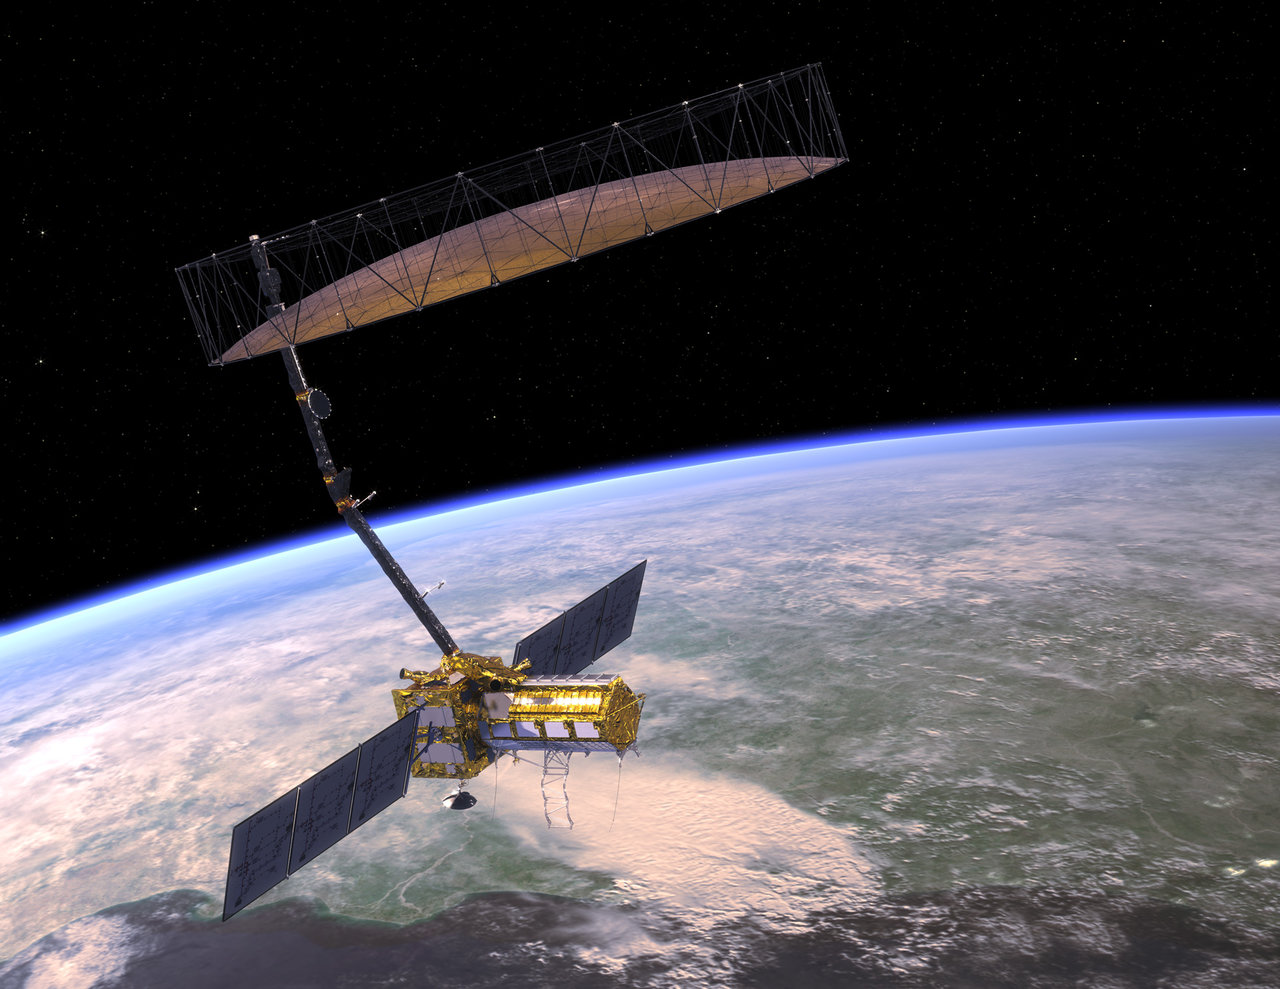
\includegraphics[scale=0.45]{Images/NISAR.jpg}
\end{figure}

\pagebreak

\section*{\Large REVISION HISTORY}

\begin{table}[h!]
\begin{center}
\begin{tabular} [0.9 \textwidth]{cl}
\hline \hline
\multicolumn{1}{c}{VERSION} & \multicolumn{1}{l}{REVISION NOTES} \\
\hline
PS1 & - Created document \\
    & - Added PS1 material \\
\hline
PS2 & - Added PS2 material \\
    & - Updated title page \\
    & - Updated moment of inertia for center of mass \\
\hline
PS3 & - Added PS3 material \\
    & - Updated title page \\
\hline
PS4 & - Added PS4 material \\
    & - Updated title page \\
    & - Switched to 312 Euler angles \\
\hline
PS5 & - Added PS5 material \\
    & - Updated title page \\
\hline \hline
\end{tabular}
	\caption{Summary of project revisions.}
\end{center}
\end{table}
 
\newpage
\section*{\Large TABLE OF CONTENTS}
\makeatletter
\@starttoc{toc}
\makeatother
\newpage
%%%%%%%%%%%%%%%%%%%%%%%%%%%%%%%%%%%%%%%%%%%%%%%%%%%%%%%%%%%%%%%%%%%%%%%%%%%%%%%%%%%%%%%%%%%%%%%%%%%%%%%%%%%%%%%%%%%%%%%%%%%%%%%%%%%%%%%%%%%%%%%%%%%%%%%%%%%%%%%%%%%%%%%%%%%%%%%%%%%%%%%%%%%%%%%%%%%%%%%%%%%%%%%%%%%%%%%%%%%

% \section{\Large INTRODUCTION}

\section{\Large PROBLEM SET 1}
\subsection{PROBLEM 1}
\textit{Select some key ADCS characteristics of your mission, including orbit (e.g., LEO, MEO, GEO, HEO, Interplanetary), target attitude (e.g., Sun pointing, Inertial pointing, Earth pointing, Resident Space Object pointing), attitude state representation (e.g., Euler angles, Gibbs vector, Quaternions Direction Cosine Matrix, Euler Axis/Angle), sensors suite (Gyros, Magnetometers, Star Trackers, Earth Sensor, Sun Sensor), actuator suite (Thrusters, Magnetorquers, Reaction Wheels, Momentum Wheel, Gravity Gradient).}

Our mission will utilize a satellite with synthetic aperture radar (SAR), designed to gather key remote sensing and environmental data for the Earth. The satellite will be in low Earth orbit (LEO) and use quaternions to describe its orientation, avoiding gimbal lock effects of other conventions. For state estimation, the spacecraft will require gyroscopes, star trackers, and a potentially a sun sensor. For actuation, the spacecraft will likely utilize thrusters, reaction wheels, and magnetorquers.

\subsection{PROBLEM 2}
\textit{Conduct survey of satellites which have characteristics similar to selected project. Use internet, publications, and books as resources.}

Space agencies such as NASA have been constructing SAR satellites to gather satellite images and data of Earth for over a decade. Additionally, there exist commercial entities also utilizing SAR in their spacecraft.

For example, Soil Moisture Active Passive (SMAP) is a NASA satellite launched in 2015 that utilizes L-band synthetic aperture radar (SAR) technology to measure soil moisture from LEO. This data has applications in climate change research climate change research applications (such as updating climate models) and some day-to-day activities (such as improving weather forecasts). SMAP is unique in that it had a large deployable reflector, held above the spacecraft body by a deployable boom \cite{SMAP}.

Companies EOS and Capella Space are also developing satellites that use SAR technology in the X-band and S-band frequencies for commercial applications ranging from agriculture to mining \cite{EOSSAR, Capella}. The commercial applicability of SAR is substantial, especially as SAR can penetrate cloud cover while generating high-resolution data, making it superior to many other forms of remote sensing technology. EOS claims to obtain resolution of up to 0.25 m, while Capella Space claims a capability of up to 0.5 m. These satellites all operate in LEO, which enables high-frequency monitoring of the Earth's surface.

NASA and ISRO have partnered to create a SAR satellite as well. The joint project between NASA JPL and ISRO has resulted in the NASA-ISRO Synthetic Aperture Radar (NISAR), a satellite that captures data in the L-band and S-band SAR frequencies \cite{NISARMission}. NISAR's high resolution will permit the detailed measurement of the Earth's surface, enabling better observation of changes in Earth's crust for disaster prevention and mitigation. NISAR will also support science goals such as monitoring ice sheets and the oceans, and its orbit is designed to cover the entire Earth every 12 days.

\subsection{PROBLEM 3}
\textit{Select preferred existing satellite and payload for project. Similarity is helpful, but not strictly required.}

We select the NASA JPL and ISRO NISAR mission as the mission on which to base our satellite. In the following section, we describe mission details and basic specifications. We simplify the satellite geometry and compute the center of mass and inertia tensor of the satellite. We will also analyze the satellite's external surfaces, which are relevant to disturbances such as atmospheric drag and solar radiation pressure.

\subsection{PROBLEM 4}
\textit{Collect basic information on mission, requirements, ADCS sensors and actuators, mechanical layout, mass, mass distribution, and inertia properties.}

NISAR is a joint Earth-observation satellite mission between NASA and ISRO. It is the first satellite to operate in two different Synthetic Aperture Radar (SAR) bands, incorportating both L- and S-band SAR instruments. Both frequencies can penetrate clouds for reliable data collection, but the L-band can also penetrate thicker vegetation that the S-band cannot. Uniquely, NISAR is intended to be used for a wide range of science objectives, including disaster response and agriculture \cite{NISARApps}.

NISAR ADCS requirements are \textless 273 arcseconds for pointing and \textless 500 m for orbit control \cite{Siqueira}. The satellite duty cycle is specified as \textgreater 30\%. NISAR will operate in LEO with nominal altitude of 747 km and 6 AM/6 PM orbit. NISAR's L- and S-band instruments operate at 24 cm and 12 cm wavelengths, respectively. NISAR collects terrestial SAR imagery with an image swatch of 240 km using a sweep approach. The science payload can also perform polarimetry, with the SAR incorporating multiple polarization modes.

\begin{figure}[H]
\centering
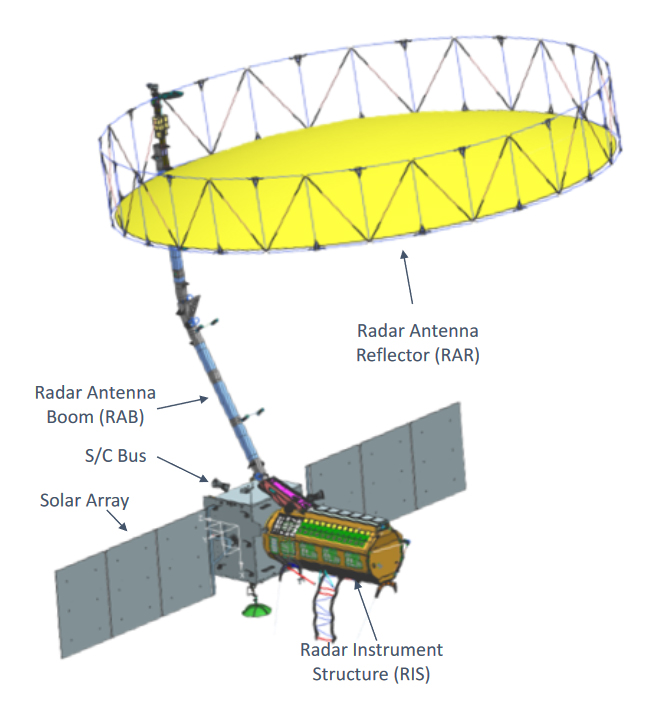
\includegraphics[scale=0.38]{Images/nisar_diagram.jpg}
\caption{The basic components of the NISAR satellite}
\label{NISAR Diagram}
\end{figure}

As shown in Figure \ref{NISAR Diagram}, NISAR's satellite consists of a 1.2 m x 1.8 m x 1.9 m spacecraft bus cuboid with a 1.2 m wide octagonal Radar Instrument Structure (RIS). The spacecraft bus includes ADCS hardware, power subsystem, and engineering payload, while the RIS houses hardware for the L- and S-band SAR. The satellite is powered by 23 m\textsuperscript{2} of solar panels, consisting of an array of two panels, one on each side of the satellite. Additionally, a 12 m diameter radar antenna is positioned above the body of the spacecraft, attached by a 9 m long boom. This boom consists of beams with 7 in x 7 in cross-section area \cite{NISARMission}.

Table \ref{tab:mass} contains mass properties of the satellite. Unfortunately, detailed mass distribution and inertia properties of NISAR are not openly available, so we provide estimates of mass distribution based on known overall component-level masses. We are given total masses for the bus structure and RIS, and we also know the masses of the payloads located within, allowing us to compute an accurate mass for these components \cite{NISARMission}. We estimate that solar panels have a mass of 23 kg each based on knowledge that NISAR's solar panels are 23 m\textsuperscript{2} and a typical solar panel mass per area is 2.06 kg/m\textsuperscript{2} \cite{SolarPanelMass}. We know that the entire radar antenna assembly has a mass of 292 kg, and we estimate that the reflector has a mass of approximately 100 kg based on a similar deployable SAR S- and L-band mesh antenna reflector \cite{L3Harris}. We will use these masses to compute center of mass and moments of inertia in the following section. For our model, we neglect the effects of the truss structure supporting the antenna reflector, instead modeling the entire RAR as just the disk-shaped reflector mesh.

\begin{longtable}{l|r}
\caption{Mass of NISAR components}
\label{tab:mass}\\
\textbf{Components}              & \multicolumn{1}{l}{\textbf{Mass [kg]}} \\ \hline
\endfirsthead
%
\endhead
%
Bus                              & 964.1                                      \\
Radar Instrument Structure (RIS) & 1375.9                                     \\
Solar Panel +y                   & 23                                         \\
Solar Panel -y                   & 23                                         \\
Radar Antenna Boom (RAB)         & 192                                        \\
Radar Antenna Reflector (RAR)    & 100                                       
\end{longtable}

Since NISAR is a remote sensing satellite requiring high attitude control performance, it has an ADCS system with an array of sensors and actuators. Sensors include star sensors, sun sensors, GPS, and a 3-axis gyroscope for roll, pitch, and yaw. For actuators, NISAR has four 50 N$\cdot$m reaction wheels mounted in tetrahedral configuration, three 565 and 350 A$\cdot$m\textsuperscript{2} magnetorquers, and fourteen thrusters (ten canted 11 N thrusters, one central 11 N thruster, and four 1 N thrusters for roll) \cite{NISARMission}.

\subsection{PROBLEM 5}
\textit{Simplify spacecraft geometry, make assumptions on mass distribution, e.g. splitting it in its core parts, define body axes (typically related to geometry and payload), compute moments of inertia and full inertia tensor w.r.t. body axes. Show your calculations.}

We simplify the spacecraft geometry into six components, each individually assumed to have uniform mass distribution. These components of the simplified geometry are: bus structure (including ADCS hardware and engineering payload), RIS (Radar Instrument Structure), RAB (radar antenna boom), RAR (radar antenna reflector), and two solar panels (identified as the +y solar panel and -y solar panel). The bus structure is modeled as a rectangular prism, while the RIS is modeled as an octagonal prism. The RAB is also modeled as a rectangular prism, while the RAR is modeled as a thin disk and the solar panels are modeled as thin rectangular plates. Within each geometry, our model assumes mass is distributed uniformly. From analyzing diagrams found in technical reports, we estimate that the RAR is tilted -3.87\degree{} about the y-axis (relative to the x-axis), while the RAB is modeled as a single beam with an angle approximately -18\degree{} from vertical (from the z-axis, about the y-axis in the x-z plane). Note that we have simplified the shape of the RAB from a beam of two angled segments to a single, straight beam.

We choose the body axes to have an origin at the center of the rectangular bus. This configuration is chosen because the bus houses the ADCS hardware, including actuators and sensors. The x-axis points in the direction of the RIS, and the z-axis points up vertically, normal to the upper surface of the bus. See Figure \ref{fig:MATLAB_model} for a visual depiction of the body axes relative to the spacecraft.

We compute the center of mass after extracting the centroid of each component. The mass of each component is previously found in Table \ref{tab:mass}. The centroid of each component is listed in Table \ref{tab:centroid}.

\begin{longtable}{l|r|r|r}
\caption{Component centroids [m]}
\label{tab:centroid}\\
\textbf{Part} & \multicolumn{1}{l}{\textbf{x}} & \multicolumn{1}{l}{\textbf{y}} & \multicolumn{1}{l}{\textbf{z}} \\ \hline
\endfirsthead
%
\endhead
%
Bus      & 0     & 0    & 0    \\
RIS      & 1.85  & 0    & 0    \\
Panel +y & 0     & 3.9  & 0    \\
Panel -y & 0     & -3.9 & 0    \\
RAB      & -0.899 & 0    & 5.194 \\
RAR      & 4.283   & 0    & 8.308
\end{longtable}

The center of mass can be found by taking the weighted average of each component centroid, weighted by the mass of each component. The center of mass formula is:

\begin{equation*}
    \Vec{r}_{cm} = \frac{\sum m_{i} \Vec{r}_{i}}{\sum m_{i}}
\end{equation*}

This yields a result for center of mass at $\qty[parse-numbers = false]{[1.046, 0, 0.683]}{\metre}$ relative to the origin we defined. We created the following MATLAB script to compute the center of mass from a CSV file containing centroid and mass data.

\lstinputlisting{src/computeCM.m}

We compute the moment of inertia of the satellite, finding an inertia tensor in our body axes. To do this, we break the satellite into individual components, first finding the moment of inertia about the center of mass of each component. We then compute the moment of inertia of the entire satellite about the body axes by using parallel axis theorem and combining all the components.

To compute the moment of inertia, we need the following geometric properties of each component:

\begin{longtable}{l|r|r|r|r|r}
\caption{Dimensions of modeled components [m]}
\label{tab:dimensions}\\
\textbf{Part} & \textbf{L (x-dim)} & \textbf{W (y-dim)} & \textbf{H (z-dim)} & \textbf{S (oct. side length)} & \textbf{R (radius)} \\ \hline
\endfirsthead
%
\endhead
%
Bus &  & 1.8 & 1.9 & - & - \\
RIS & 2.5 & - & - & 0.459 & - \\
Panel +y & - & 6 & 1.9 & - & - \\
Panel -y & - & 6 & 1.9 & - & - \\
RAB & 0.1778 & 0.1778 & 9 & - & - \\
RAR & - & - & - & - & 6
\end{longtable}

For the bus, we choose to model the geometry as a rectangular prism. Since the bus is aligned with the body axes, we obtain a diagonal inertia tensor:

\begin{align*}
I_{bus} &=
\begin{bmatrix}
I_{xx} & 0 & 0 \\
0 & I_{yy} & 0 \\
0 & 0 & I_{zz}
\end{bmatrix} \\
&=
\begin{bmatrix}
m \frac{W^{2} + H^{2}}{12} & 0 & 0 \\
0 & m \frac{L^{2} + H^{2}}{12} & 0 \\
0 & 0 & m \frac{L^{2} + W^{2}}{12} 
\end{bmatrix} \\
&=
\qty[parse-numbers = false]{
\begin{bmatrix}
550.340 & 0 & 0 \\
0 & 405.725 & 0 \\
0 & 0 & 375.9993 
\end{bmatrix}
}{\kilogram\metre\squared}
\end{align*}

For the solar panels, we approximate their geometry as a flat plate. These axes are also aligned, so the tensor can be diagonal.

\begin{align*}
I_{panel} &=
\begin{bmatrix}
I_{xx} & 0 & 0 \\
0 & I_{yy} & 0 \\
0 & 0 & I_{zz}
\end{bmatrix} \\
&=
\begin{bmatrix}
m \frac{W^{2} + H^{2}}{12} & 0 & 0 \\
0 & m \frac{H^{2}}{12} & 0 \\
0 & 0 & m \frac{W^{2}}{12} 
\end{bmatrix} \\
&=
\qty[parse-numbers = false]{
\begin{bmatrix}
75.919 & 0 & 0 \\
0 & 6.919 & 0 \\
0 & 0 & 69 
\end{bmatrix}
}{\kilogram\metre\squared}
\end{align*}

For the RIS, we model the geometry as an octagonal prism. For the moment of inertia about the axisymmetric axis of the octagon, we use the formula $m \left(\frac{S^{2}}{24} + \frac{a^{2}}{2}\right)$, where $S$ is the side length and $a$ is the apothem length, where the apothem is the perpendicular length from a side of the octagon to the center \cite{McCarron}. When calculating the moment of inertia about the non-axisymmetric axes, we approximate the geometry as a cylinder with radius equal to the average of the octagonal radius (distance from center to vertex) and the apothem. As will be shown later, this approximation yields a very close result to the inertia tensor generated from the CAD model.

\begin{align*}
I_{RIS} &=
\begin{bmatrix}
I_{xx} & 0 & 0 \\
0 & I_{yy} & 0 \\
0 & 0 & I_{zz}
\end{bmatrix} \\
&=
\begin{bmatrix}
m \left(\frac{S^{2}}{24} + \frac{a^{2}}{2}\right) & 0 & 0 \\
0 & m \left(\frac{L^{2}}{12} + \frac{R_{avg}^{2}}{4}\right) & 0 \\
0 & 0 & m \left(\frac{L^{2}}{12} + \frac{R_{avg}^{2}}{4}\right) 
\end{bmatrix} \\
&=
\qty[parse-numbers = false]{
\begin{bmatrix}
223.268 & 0 & 0 \\
0 & 831.089 & 0 \\
0 & 0 & 831.089 
\end{bmatrix}
}{\kilogram\metre\squared}
\end{align*}

For the RAB, we first model the geometry as a rectangular prism. We also must rotate the inertia tensor to match the orientation of the body axes, as the RAB itself is rotated relative to the bus about the y-axis by -18\degree{} from vertical (z-axis).

\begin{align*}
I_{RAB} &=
\begin{bmatrix}
I_{xx} & 0 & 0 \\
0 & I_{yy} & 0 \\
0 & 0 & I_{zz}
\end{bmatrix} \\
&=
\begin{bmatrix}
m \frac{W^{2} + H^{2}}{12} & 0 & 0 \\
0 & m \frac{L^{2} + H^{2}}{12} & 0 \\
0 & 0 & m \frac{L^{2} + W^{2}}{12} 
\end{bmatrix} \\
&=
\qty[parse-numbers = false]{
\begin{bmatrix}
1296.506 & 0 & 0 \\
0 & 1296.506 & 0 \\
0 & 0 & 1.012 
\end{bmatrix}
}{\kilogram\metre\squared}
\end{align*}

We apply the rotation to the inertia tensor using a rotation matrix about the y-axis. Note that doing so results in non-zero products of inertia, meaning our principal axes will not be aligned with our body axes.

\begin{align*}
I_{RAB,rotated} &= R_{y}(-18\degree) I_{RAB} R_{y}^{\intercal}(-18\degree) \\
&=
\qty[parse-numbers = false]{
\begin{bmatrix}
1172.797 & 0 & 380.736 \\
0 & 1296.506 & 0 \\
380.736 & 0 & 124.720
\end{bmatrix}
}{\kilogram\metre\squared}
\end{align*}

Finally, we model the RAR as a flat disk. Similar to the RAB, we must rotate the inertia tensor to match the orientation of the body axes.

\begin{align*}
I_{RAR} &=
\begin{bmatrix}
I_{xx} & 0 & 0 \\
0 & I_{yy} & 0 \\
0 & 0 & I_{zz}
\end{bmatrix} \\
&=
\begin{bmatrix}
m \frac{R^{2}}{4} & 0 & 0 \\
0 & m \frac{R^{2}}{4} & 0 \\
0 & 0 & m \frac{R^{2}}{2} 
\end{bmatrix} \\
&=
\qty[parse-numbers = false]{
\begin{bmatrix}
900 & 0 & 0 \\
0 & 900 & 0 \\
0 & 0 & 1800 
\end{bmatrix}
}{\kilogram\metre\squared}
\end{align*}

Applying a rotation:

\begin{align*}
I_{RAR,rotated} &= R_{y}(-3.87\degree) I_{RAR} R_{y}^{\intercal}(-3.87\degree) \\
&=
\qty[parse-numbers = false]{
\begin{bmatrix}
904.100 & 0 & -60.605 \\
0 & 900 & 0 \\
-60.605 & 0 & 1795.900
\end{bmatrix}
}{\kilogram\metre\squared}
\end{align*}

Now, we use parallel axis theorem to compute the moment of inertia of each component about the body axes at the specified origin. We can use the following displacement tensor,

\begin{equation*}
D =
\begin{bmatrix}
y^{2} + z^{2} & -xy & -xz \\
-yx & x^{2} + z^{2} & -yz \\
-zx & -yz & x^{2} + y^{2}
\end{bmatrix},
\end{equation*}

where $x$, $y$, $z$ are the coordinates of the center of mass of the component, giving the moment of inertia about a new point:

\begin{equation*}
    I' = I_{c} + mD
\end{equation*}

Performing the parallel axis theorem on each component and summing the inertia tensors, we obtain the following inertia tensor for the entire spacecraft:

\begin{equation*}
I_{NISAR,body} =
\qty[parse-numbers = false]{
\begin{bmatrix}
15783.996 & 0 & -2341.659 \\
0 & 22227.752 & 0 \\
-2341.659 & 0 & 10663.970
\end{bmatrix}
}{\kilogram\metre\squared}
\end{equation*}

Compare this with the inertia tensor computed by SolidWorks CAD software:

\begin{equation*}
I_{NISAR,body} =
\qty[parse-numbers = false]{
\begin{bmatrix}
15780.361 & 0 & -2336.285 \\
0 & 22225.721 & 0 \\
-2336.285 & 0 & 10665.796
\end{bmatrix}
}{\kilogram\metre\squared}
\end{equation*}

The errors are 0.0230\%, 0.00914\%, 0.0171\%, and 0.230\% for $I_{xx}$, $I_{yy}$, $I_{zz}$, and $I_{xz}$, respectively. We created the following MATLAB script to compute the inertia tensor.

\lstinputlisting{src/computeMOI.m}

\subsection{PROBLEM 6}
\textit{Discretize your spacecraft through its outer surfaces (geometry). Develop a Matlab/Simulink function to handle barycenter (geometry, no mass distribution) coordinates, size, and unit vectors normal to each outer surface of the spacecraft in body frame. You can list all this information in a Matrix. This will be essential later on to compute environmental torques acting on the spacecraft from forces, surface orientation, and the vectors connecting the satellite’s center of mass to each surface’s center of mass.}

For the purpose of discretizing the spacecraft into surfaces, we consider the outer faces of the bus, RIS, and RAB. We also consider the faces of the solar panels and RAR, which are modeled as thin plates. The centroid (barycenter) coordinates and area for each surface are obtained using the surface properties tool in SolidWorks, and a unit normal vector is manually computed based on the orientation of the surface. We then enter this data into a CSV file, which can be read into MATLAB using the following function:

\lstinputlisting{src/surfaces.m}

This function stores the data into arrays of barycenter coordinates, unit normal vector components, and area. Each row of an array corresponds to a particular surface. The data is shown in Table \ref{tab:surfaces}, annotated with the identity of each surface.

\begin{longtable}{l|r|r|r|r|r|r|r}
\caption{Surface parameters}
\label{tab:surfaces}\\
 &
  \multicolumn{3}{c}{\textbf{Barycenter [m]}} &
  \multicolumn{3}{c}{\textbf{Normal}} &
  \multicolumn{1}{l}{} \\
\endfirsthead
%
\endhead
%
\textbf{Surface} &
  \multicolumn{1}{l}{\textbf{x}} &
  \multicolumn{1}{l}{\textbf{y}} &
  \multicolumn{1}{l}{\textbf{z}} &
  \multicolumn{1}{l}{\textbf{x}} &
  \multicolumn{1}{l}{\textbf{y}} &
  \multicolumn{1}{l}{\textbf{z}} &
  \multicolumn{1}{l}{\textbf{Area [m\textsuperscript{2}]}} \\ \hline
Bus front, minus RIS (+x) & 0.6   & 0     & 0     & 1      & 0      & 0      & 2.4   \\
Bus rear (-x)                  & -0.6  & 0     & 0     & -1     & 0      & 0      & 3.42  \\
Bus side (+y)                  & 0     & 0.9   & 0     & 0      & 1      & 0      & 2.28  \\
Bus side (-y)                  & 0     & -0.9  & 0     & 0      & -1     & 0      & 2.28  \\
Bus top (+z)                   & 0     & 0     & 0.95  & 0      & 0      & 1      & 2.16  \\
Bus bottom (-z)                & 0     & 0     & -0.95 & 0      & 0      & -1     & 2.16  \\
RIS front (+x)                 & 3.1   & 0     & 0     & 1      & 0      & 0      & 1.02  \\
RIS top (+z)                   & 1.85  & 0     & 0.55  & 0      & 0      & 1      & 1.15  \\
RIS bottom (-z)                & 1.85  & 0     & -0.55 & 0      & 0      & -1     & 1.15  \\
RIS side (+y)                  & 1.85  & 0.55  & 0     & 0      & 1      & 0      & 1.15  \\
RIS side (-y)                  & 1.85  & -0.55 & 0     & 0      & -1     & 0      & 1.15  \\
RIS angle face (y-z I)         & 1.85  & 0.39  & 0.39  & 0      & 0.707  & 0.707  & 1.15  \\
RIS angle face (y-z II)        & 1.85  & -0.39 & 0.39  & 0      & -0.707 & 0.707  & 1.15  \\
RIS angle face (y-z III)       & 1.85  & -0.39 & -0.39 & 0      & -0.707 & -0.707 & 1.15  \\
RIS angle face (y-z IV)        & 1.85  & 0.39  & -0.39 & 0      & 0.707  & -0.707 & 1.15  \\
Panel +y front (+x)            & 0     & 3.9   & 0     & 1      & 0      & 0      & 11.4  \\
Panel +y rear (-x)             & 0     & 3.9   & 0     & -1     & 0      & 0      & 11.4  \\
Panel -y front (+x)            & 0     & -3.9  & 0     & 1      & 0      & 0      & 11.4  \\
Panel -y rear (-x)             & 0     & -3.9  & 0     & -1     & 0      & 0      & 11.4  \\
RAB front (x-z, +x)            & -0.81 & 0     & 5.21  & 0.951  & 0      & 0.309  & 1.6   \\
RAB rear (x-z, -x)             & -0.99 & 0     & 5.18  & -0.951 & 0      & -0.309 & 1.6   \\
RAB side (+y)                  & -0.9  & -0.09 & 5.19  & 0      & 1      & 0      & 1.6   \\
RAB side (-y)                  & -0.9  & 0.09  & 5.19  & 0      & -1     & 0      & 1.6   \\
RAB top (+z)                   & -2.31 & 0     & 9.47  & 0      & 0      & 1      & 0.03  \\
RAR top (+z)                   & 4.28  & 0     & 8.31  & -0.067 & 0      & 0.998  & 113.1 \\
RAR bottom (-z)                & 4.28  & 0     & 8.31  & 0.067  & 0      & -0.998 & 113.1
\end{longtable}

\subsection{PROBLEM 7}
\textit{At this stage you should have a simple 3D model of your spacecraft including geometry and mass properties of each element. Plot body axes (triad) in 3D superimposed to spacecraft 3D model.}



A 3D model of the spacecraft is shown in Figure \ref{fig:complex_model}. The model shown is a screen capture from the SolidWorks CAD software.

\begin{figure}[H]
\centering
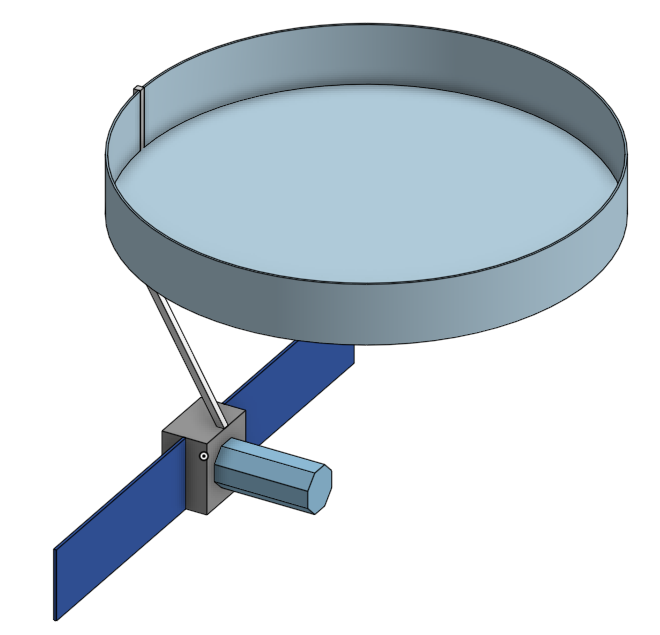
\includegraphics[scale=0.4]{Images/ps1_complex_model.png}
\caption{A 3D model of the satellite}
\label{fig:complex_model}
\end{figure}


We also show a simplified model of the spacecraft in Figure \ref{fig:simple_model}. This is the model we use to compute our mass and surface properties.

\begin{figure}[H]
\centering
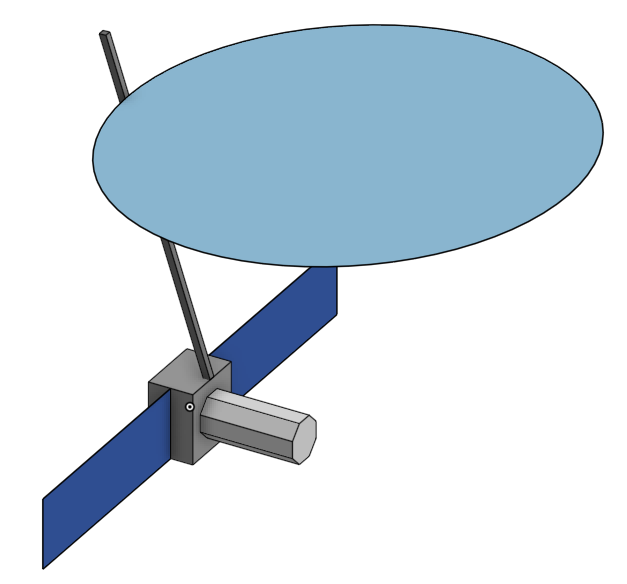
\includegraphics[scale=0.4]{Images/ps1_simple_model.png}
\caption{A 3D model of the simplified satellite geometry}
\label{fig:simple_model}
\end{figure}

We also plot the model in MATLAB by importing an STL version of the CAD model. We show the body axes in Figure \ref{fig:MATLAB_model}, with the origin chosen as the center of the spacecraft bus.

\begin{figure}[H]
\centering
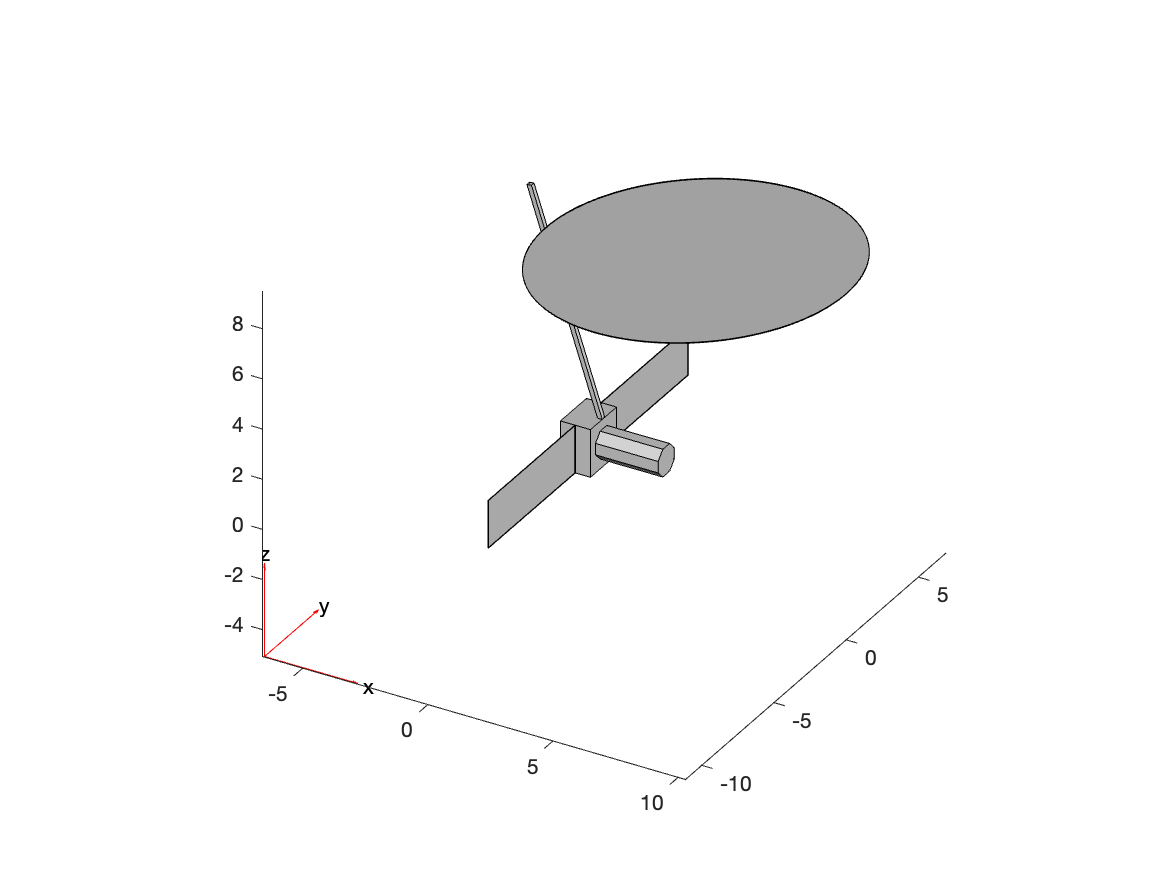
\includegraphics[scale=0.7]{Images/ps1_model.png}
\caption{Satellite model in MATLAB with body axes shown}
\label{fig:MATLAB_model}
\end{figure}



\section{\Large PROBLEM SET 2}
\subsection{PROBLEM 1}
\textit{Define orbit initial conditions and make sure you can propagate the orbit of the satellite over multiple orbits using either a Keplerian propagator or a numerical integration scheme (see AA279A material). Best would be to use a numerical integrator, so that you can later try to feed the same environmental forces for orbit propagation which are applied for attitude propagation (very cool!).}

From the science users' handbook, we obtain the following orbital elements \cite{NISARHandbook}.

\begin{table}[H]
\begin{tabular}{lllllll}
\textbf{OE} & \textit{a} & \textit{e} & \textit{i} & \textit{$\Omega$} & \textit{$\omega$} & \textit{$\nu$} \\ \hline
\textbf{Value} & 7125.48662 km & 0.0011650 & 98.40508$\degree$ & -19.61601$\degree$ & 89.99764$\degree$ & -89.99818$\degree$
\end{tabular}
\end{table}

We convert these using a MATLAB function into ECI coordinates that can be fed into a numerical orbital propagator. Notice that we first convert the orbital elements a, e, and $\nu$ into perifocal (PQW) coordinates, using a and e to find the semi-latus rectum and a, e, and $\nu$ to find the distance to the central body (Earth). Then, we perform a series of rotations on these coordinates parameterized by $\omega$, i, and $\Omega$ to obtain new coordinates in the ECI frame.

\lstinputlisting{src/oe2eci.m}

Then, we can numerically propagate in MATLAB using \texttt{ode113} using a function that computes the time derivative of the ECI state. This is accomplished simply by setting the time derivative of position equal to the velocity portion of the state and setting the time derivative of velocity equal to an acceleration computed using the law of universal gravitation. Note that while our propagator does not include disturbance forces, it will be easy to incorporate these later. See the appendix corresponding to Problem Set 2 for application of \texttt{ode113}.

\lstinputlisting{src/orbitSimple.m}

Now, we plot the trajectory for one orbit in Figure \ref{fig:simple_propagator}. Plotting multiple orbits (for example, over 12 days) yields the same plot, as \texttt{ode113} is very stable for this application.

\begin{figure}[H]
\centering
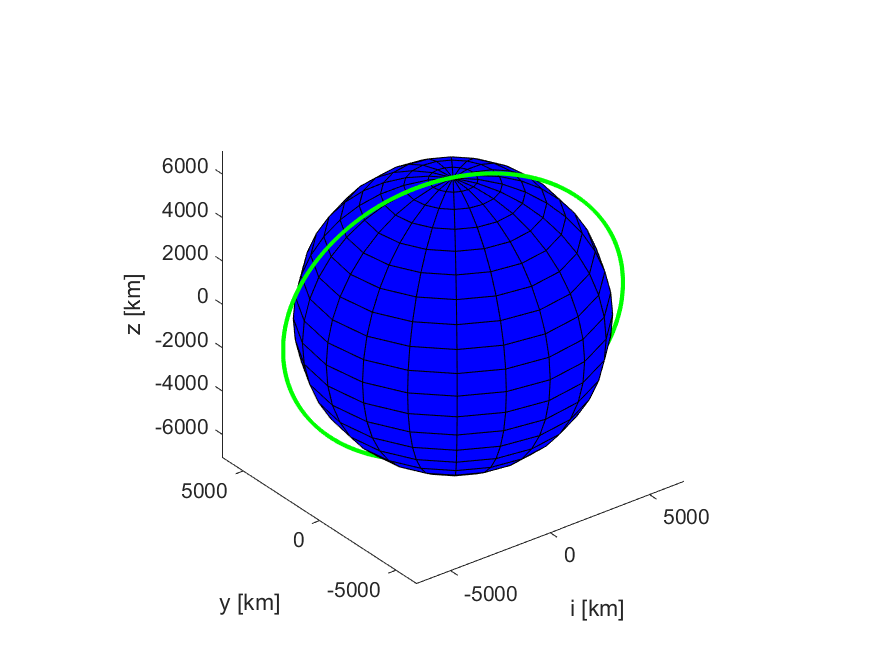
\includegraphics[scale=0.7]{Images/ps2_problem1.png}
\caption{A single orbit for NISAR in ECI coordinates (no perturbations)}
\label{fig:simple_propagator}
\end{figure}


\subsection{PROBLEM 2}
\textit{In general the body axes are not the principal axes. Identify principal axes through the eigenvector/eigenvalue problem discussed in class and compute the rotation matrix from body to principal axes.}

The unit vectors of the principal axes with respect to the body axes ($\Vec{e}_i$) and the inertia tensor in the principal axes ($I_i$) can be found by taking the eigenvalue decomposition of the inertia tensor in the body axis. This can be seen in the two equations below.

\begin{equation*}
    I_i \cdot \Vec{e}_i = I_i \cdot \Vec{I}_{body} \\ \hspace{1cm} i = x, y, z
\end{equation*}

\begin{align*}
\Vec{I}_{principal} &= 
    \begin{bmatrix}
    I_x & 0 & 0 \\
    0 & I_y & 0 \\
    0 & 0 & I_z 
    \end{bmatrix}
= 
\qty[parse-numbers = false]{
    \begin{bmatrix}
    7707.07 & 0 & 0 \\
    0 & 14563.2 & 0 \\
    0 & 0 & 18050.4 
    \end{bmatrix}
}{\kilogram\metre\squared}
\end{align*}

We follow convention $I_z > I_y > I_x$ for defining principal axes.

The unit vectors of the principal axes ($\Vec{e}_i$) can then be used to find the rotation matrix ($\Vec{R}$), as shown below.

\begin{align*}
\Vec{R} &= 
    \begin{bmatrix}
    \Vec{e}_x & \Vec{e}_y & \Vec{e}_z 
    \end{bmatrix}
= 
    \begin{bmatrix}
    -0.06278 & -0.99803 & 0 \\
    0 & 0 & 1 \\
    -0.99803 & 0.06278 & 0 
    \end{bmatrix} \\
    \Vec{I}_{body} &= \Vec{R} \Vec{I}_{principal} \Vec{R}^{\intercal}
\end{align*}


\subsection{PROBLEM 3}
\textit{At this stage you should have a simple 3D model of your spacecraft including geometry and mass properties of each element. This includes at least two coordinate systems, body and principal axes respectively, and the direction cosine matrix between them. Plot axes of triads in 3D superimposed to spacecraft 3D model.}

\begin{figure}[H]
\centering
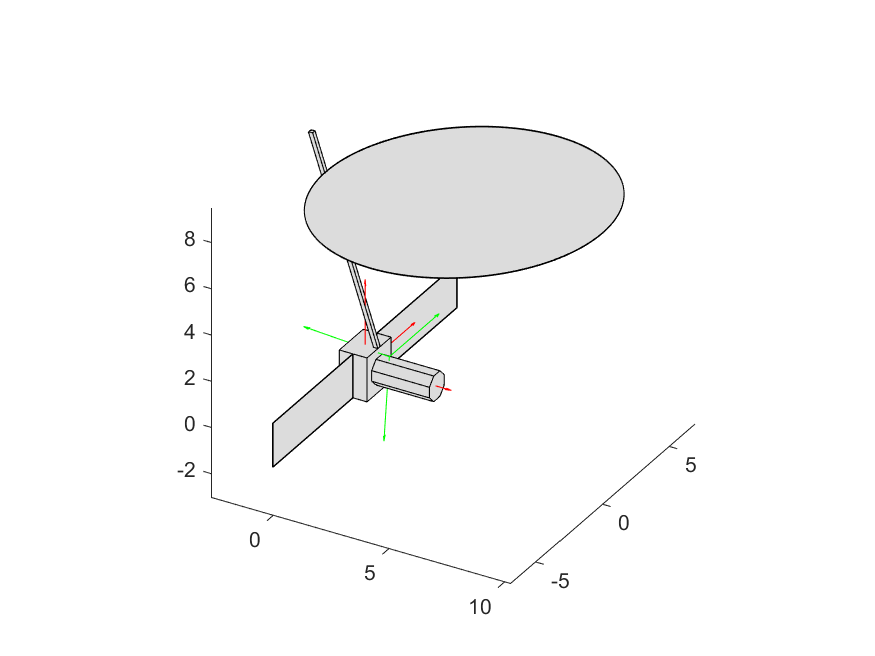
\includegraphics[scale=0.7]{Images/ps2_model.png}
\caption{Principal axes at center of mass (green) and body axes at origin (red)}
\label{fig:ps2_model}
\end{figure}


\subsection{PROBLEM 4}
\textit{Program Euler equations in principal axes (e.g. in Matlab/Simulink). No external torques.}

We use the following equations with zero external moments ($M_{x}, M_{y}, M_{z} = 0$).

\begin{align*}
    I_{x} \Dot{\omega}_{x} + (I_{z} - I_{y}) \omega_{y} \omega_{z} &= M_{x} \\
    I_{y} \Dot{\omega}_{y} + (I_{x} - I_{z}) \omega_{z} \omega_{x} &= M_{y} \\
    I_{z} \Dot{\omega}_{z} + (I_{y} - I_{x}) \omega_{x} \omega_{y} &= M_{z}
\end{align*}

\lstinputlisting{src/eulerEquation.m}


\subsection{PROBLEM 5}
\textit{Numerically integrate Euler equations from arbitrary initial conditions ($\omega<\qty{10}{\degree/\second}$, $\omega_{i}\neq0$). Multiple attitude revolutions.}

We choose arbitrary initial conditions $\omega_{x} = \qty{8}{\degree\per\second}$, $\omega_{y} = \qty{4}{\degree\per\second}$, and $\omega_{z} = \qty{6}{\degree\per\second}$. The results of numerical integration using \texttt{ode113} are shown in Figure \ref{fig:ps2_euler_equations}.

\begin{figure}[H]
\centering
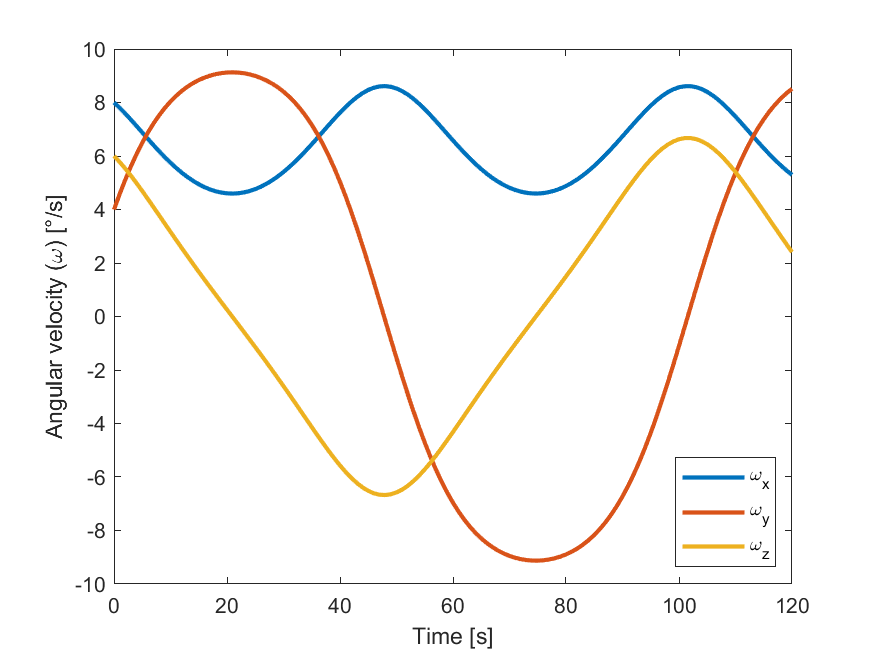
\includegraphics[scale=0.6]{Images/ps2_euler_equations.png}
\caption{Results from numerical integration of Euler equations}
\label{fig:ps2_euler_equations}
\end{figure}


\subsection{PROBLEM 6}
\textit{Plot rotational kinetic energy and momentum ellipsoids in 3D (axis equal) corresponding to chosen initial conditions. Verify that semi-axis of ellipsoids corresponds to theoretical values.}

For the energy ellipsoid, we compute our surface using rotational kinetic energy based on initial conditions and principal axes inertia tensor.

\begin{align*}
    &2T = \omega_{x}^{2} I_{x} + \omega_{y}^{2} I_{y} + \omega_{z}^{2} I_{z} \\
    &\frac{\omega_{x}^{2}}{2T/I_{x}} + \frac{\omega_{y}^{2}}{2T/I_{y}} + \frac{\omega_{z}^{2}}{2T/I_{z}} = 1
\end{align*}

For the given initial conditions, we get semi-major axes of the following lengths: $\omega_{x} = \qty{0.2332}{\radian\per\second}$, $\omega_{y} = \qty{0.1697}{\radian\per\second}$, and $\omega_{z} = \qty{0.1524}{\radian\per\second}$. These values make sense given the equation for the energy ellipsoid.

Similarly, we compute our surface for the momentum ellipsoid with angular momentum based on our initial conditions and the principal axes inertia tensor.

\begin{align*}
    &L = \omega_{x}^{2} I_{x}^{2} + \omega_{y}^{2} I_{y}^{2} + \omega_{z}^{2} I_{z}^{2} \\
    &\frac{\omega_{x}^{2}}{(L/I_{x})^{2}} + \frac{\omega_{y}^{2}}{(L/I_{y})^{2}} + \frac{\omega_{z}^{2}}{(L/I_{z})^{2}} = 1
\end{align*}

For the given initial conditions, we get semi-major axes of the following lengths: $\omega_{x} = \qty{0.3115}{\radian\per\second}$, $\omega_{y} = \qty{0.1649}{\radian\per\second}$, and $\omega_{z} = \qty{0.1330}{\radian\per\second}$. These values make sense given the equation for the momentum ellipsoid and are shown in the plots below.

We plot the energy ellipsoid in Figure \ref{fig:ps2_problem6_energy} and the momentum ellipsoid in Figure \ref{fig:ps2_problem6_momentum}.

\begin{figure}[H]
\centering
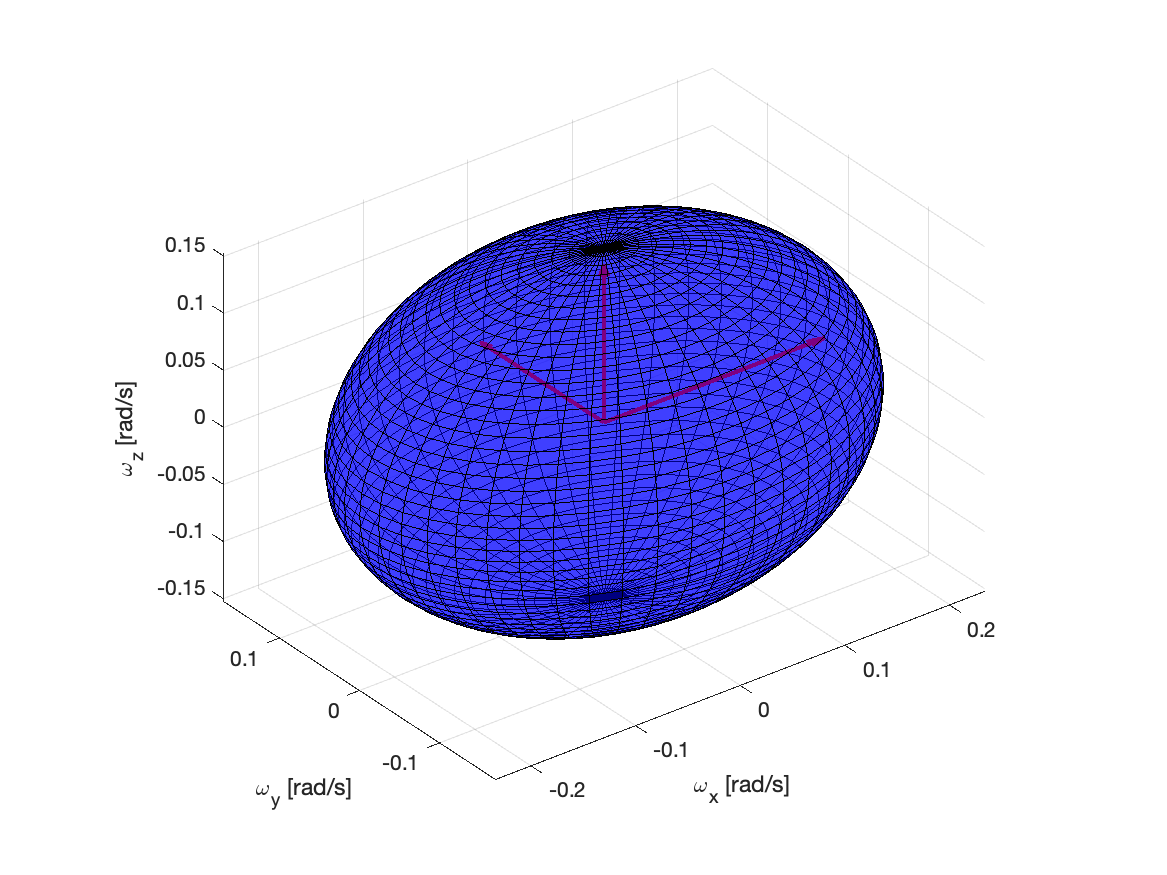
\includegraphics[scale=0.5]{Images/ps2_problem6_energy.png}
\caption{Energy ellipsoid with axes in red}
\label{fig:ps2_problem6_energy}
\end{figure}

\begin{figure}[H]
\centering
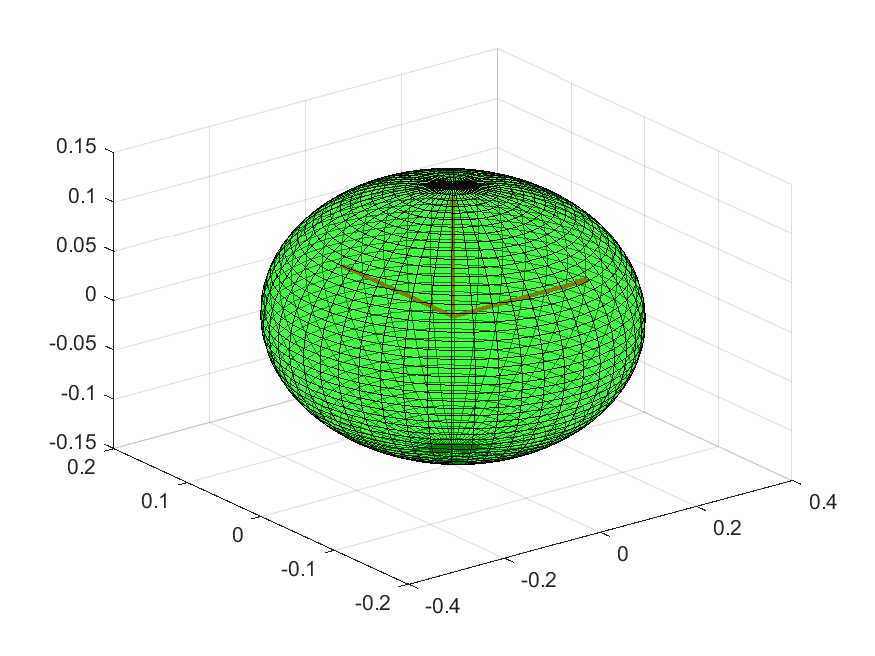
\includegraphics[scale=0.5]{Images/ps2_problem6_momentum.png}
\caption{Momentum ellipsoid with axes in red}
\label{fig:ps2_problem6_momentum}
\end{figure}


\subsection{PROBLEM 7}
\textit{Plot polhode in same 3D plot. Verify that it is the intersection between the ellipsoids.}

For a polhode plot to be real, the condition below must be verified.

\begin{equation*}
    I_x < \frac{L^2}{2T} < I_z
\end{equation*}

Based on previously calculated values ($I_x = 7707.1$, $\frac{L^2}{2T} = 13752.1$, $I_z = 18050.4$) we can verify that the polhode here will be real.

Figure \ref{fig:ps2_problem8} shows that the polhode is indeed the intersection between the ellipsoids.

\begin{figure}[H]
\centering
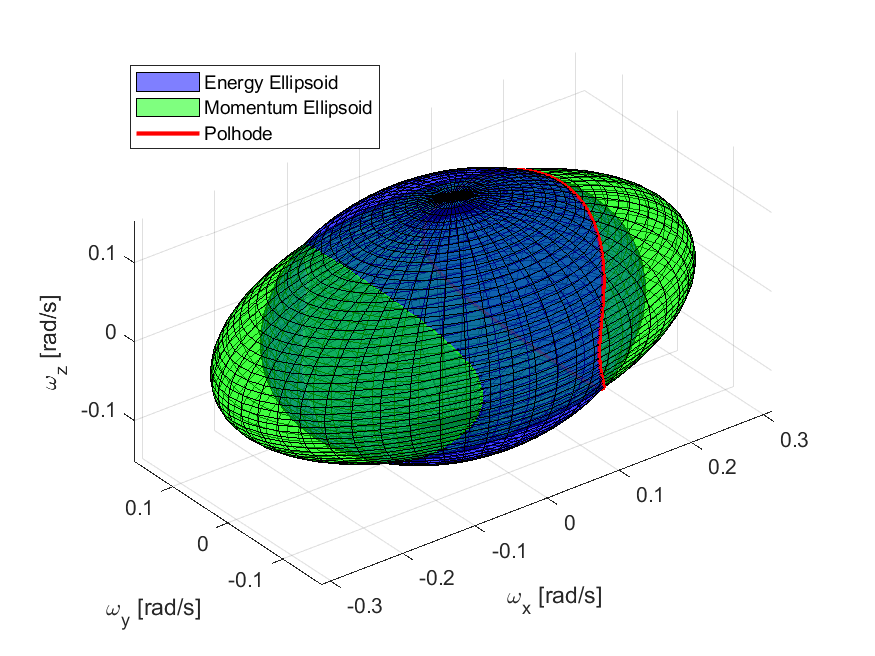
\includegraphics[scale=0.65]{Images/ps2_problem7.png}
\caption{Energy and momentum ellipsoids with polhode}
\label{fig:ps2_problem7}
\end{figure}

\subsection{PROBLEM 8}
\textit{Plot polhode in three 2D planes identified by principal axes (axis equal). Verify that shapes of resulting conic sections correspond to theory.}

The polhode conic sections in Figure \ref{fig:ps2_problem8} match expected theory. The polhode as seen along the x-axis is an ellipse, while the polhode along the y-axis is a hyperbola. We also see that when seen along the z-axis, the polhode also forms an ellipse, shown as a half-ellipse in our plot.

\begin{figure}[H]
\centering
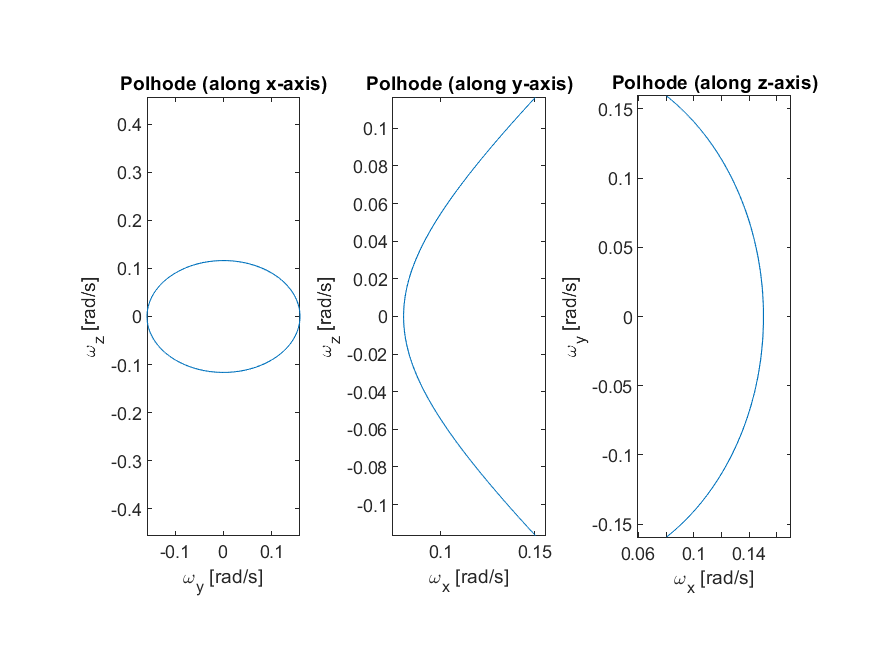
\includegraphics[scale=0.7]{Images/ps2_problem8.png}
\caption{2D views of polhode}
\label{fig:ps2_problem8}
\end{figure}


\subsection{PROBLEM 9}
\textit{Repeat above steps changing initial conditions, e.g. setting angular velocity vector parallel to principal axis. Is the behavior according to expectations?}

We show the angular velocity evolution with the initial conditions shown in Table \ref{tab:ps2_problem9_conditions}. Case 1 involves rotation about the principal x-axis, Case 2 involves rotation about the principal y-axis with a slight disturbance, and Case 3 involved rotation about the z-axis with a slight disturbance.

\begin{table}[H]
\centering
\label{tab:ps2_problem9_conditions}
\begin{tabular}{|l|l|l|l|}
\hline
\textbf{Case} & \textbf{$\omega_x$ (deg/s)} & \textbf{$\omega_y$ (deg/s)} & \textbf{$\omega_z$ (deg/s)} \\ \hline
1             & 8                     & 0                     & 0                     \\ \hline
2             & 0.08                  & 8                     & 0.08                  \\ \hline
3             & 0.08                  & 0                     & 8                     \\ \hline
\end{tabular}
\end{table}

The specifics of Case 1 are shown in the angular velocity plot in Figure \ref{fig:ps2_problem9_euler_equations_x}, the polhode and ellipsoids in Figure \ref{fig:ps2_problem9_p7_x}, and the 2D views of the polhode in Figure \ref{fig:ps2_problem9_p8_x}. The behavior shown is as expected–when the angular velocity is parallel to the principal axis, we do not have coupling with the other components of angular velocity, and the polhode views in 2D become points rather than conic sections.

For Case 2, Figure \ref{fig:ps2_problem9_euler_equations_y} shows that the satellite's rotational behavior will oscillate as expected, owing to the properties of the intermediate axis. Additionally, Figure \ref{fig:ps2_problem9_p7_y}, and the 2D views in Figure \ref{fig:ps2_problem9_p8_y} show a larger polhode, with the slight disturbances leading to ellipsoids with a substantial intersection. Interestingly, there seems to be a very sharp hyperbola in the xz-plane of the polhode.

Figure \ref{fig:ps2_problem9_euler_equations_z} illustrates a slight oscillation of angular velocities about the x- and y-axes in Case 3. Meanwhile, the actual region of intersection in the polhode as shown in Figures \ref{fig:ps2_problem9_p7_z} and \ref{fig:ps2_problem9_p8_z} is much smaller than in other cases, but not a single point like in the Case 1.

\begin{figure}[H]
\centering
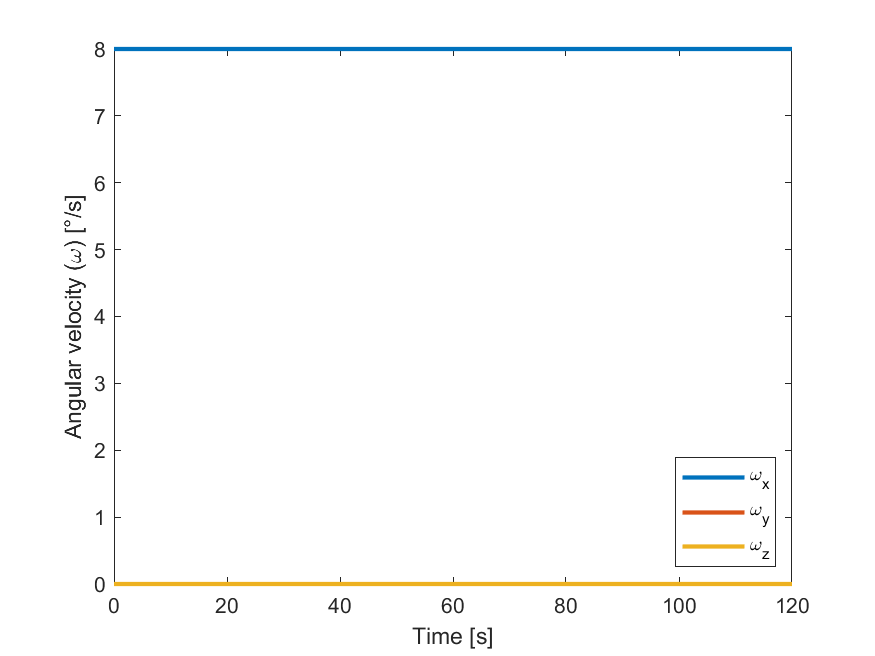
\includegraphics[scale=0.6]{Images/ps2_problem9_euler_equations_x.png}
\caption{Angular velocity evolution for angular velocity vector for Case 1}
\label{fig:ps2_problem9_euler_equations_x}
\end{figure}

\begin{figure}[H]
\centering
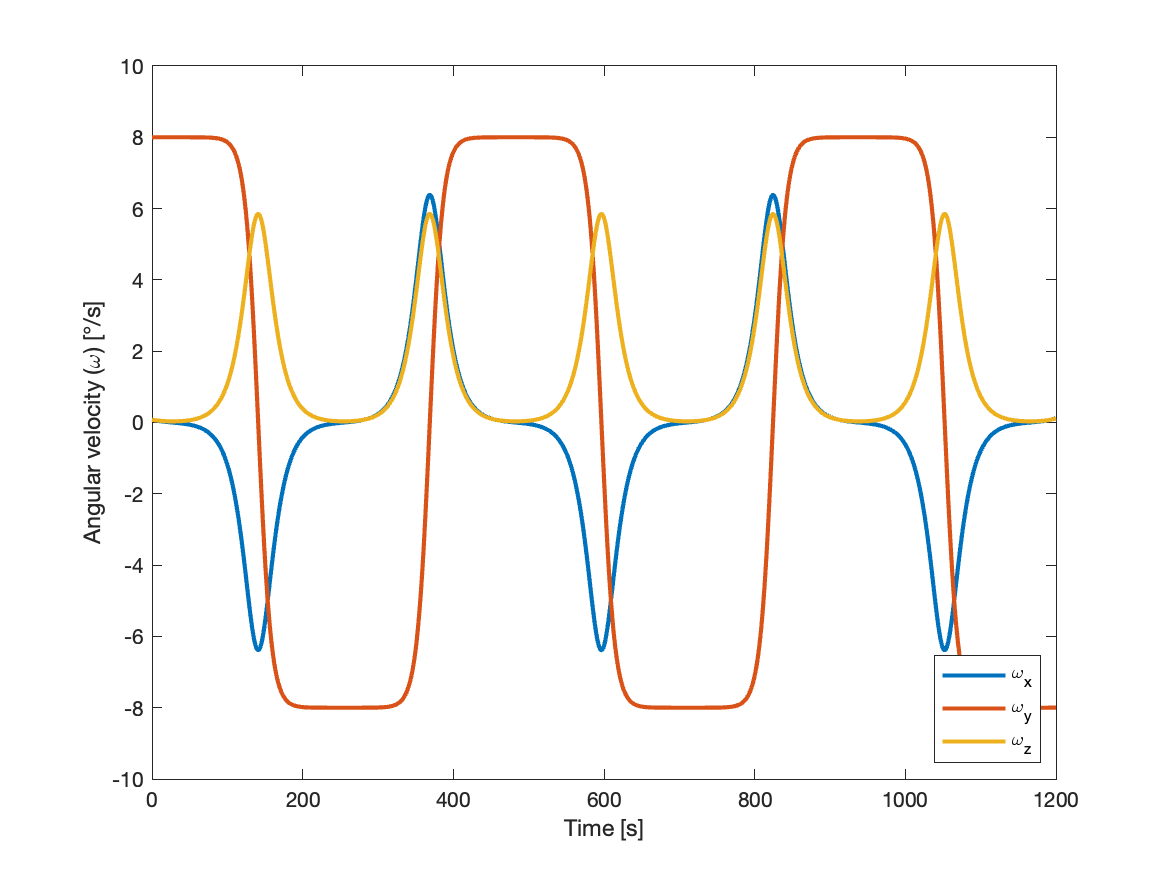
\includegraphics[scale=0.6]{Images/ps2_problem9_euler_equations_y.png}
\caption{Angular velocity evolution for angular velocity vector for Case 2}
\label{fig:ps2_problem9_euler_equations_y}
\end{figure}

\begin{figure}[H]
\centering
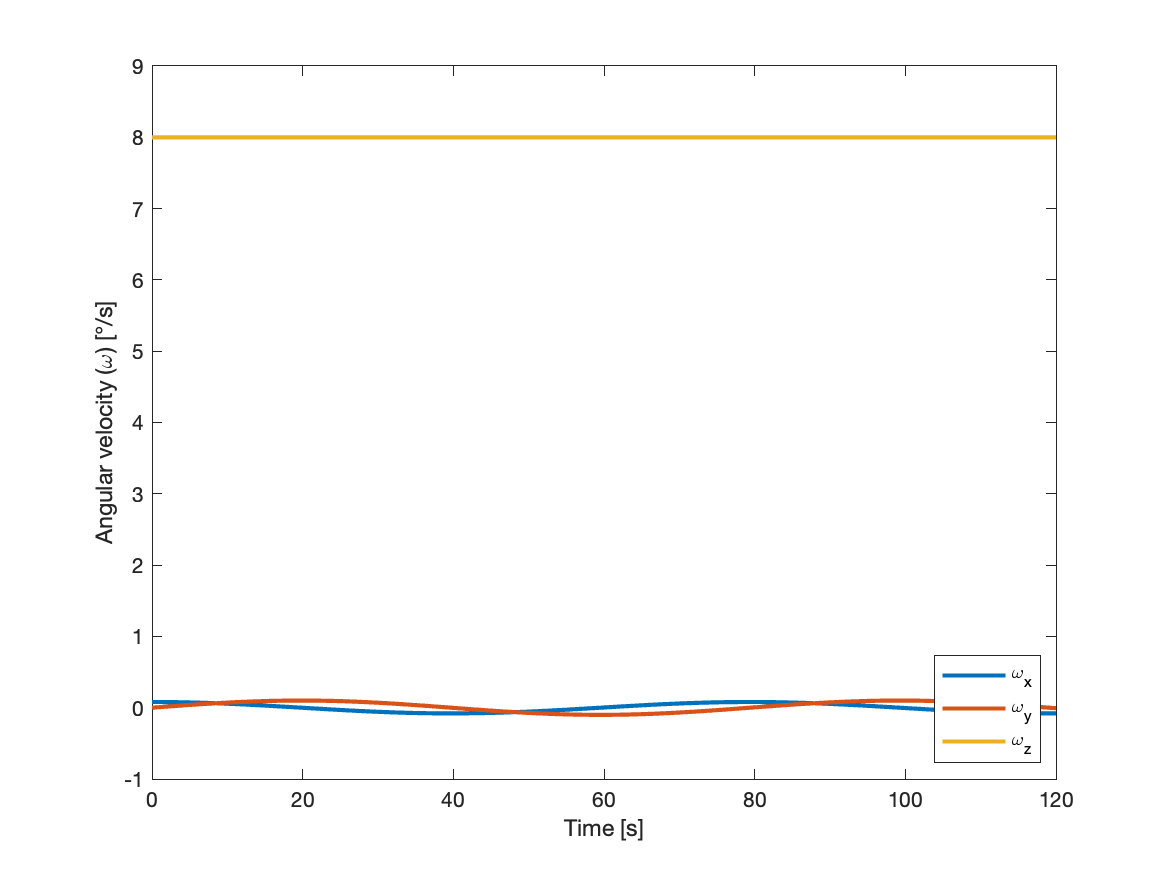
\includegraphics[scale=0.6]{Images/ps2_problem9_euler_equations_z.png}
\caption{Angular velocity evolution for angular velocity vector for Case 3}
\label{fig:ps2_problem9_euler_equations_z}
\end{figure}

\begin{figure}[H]
\centering
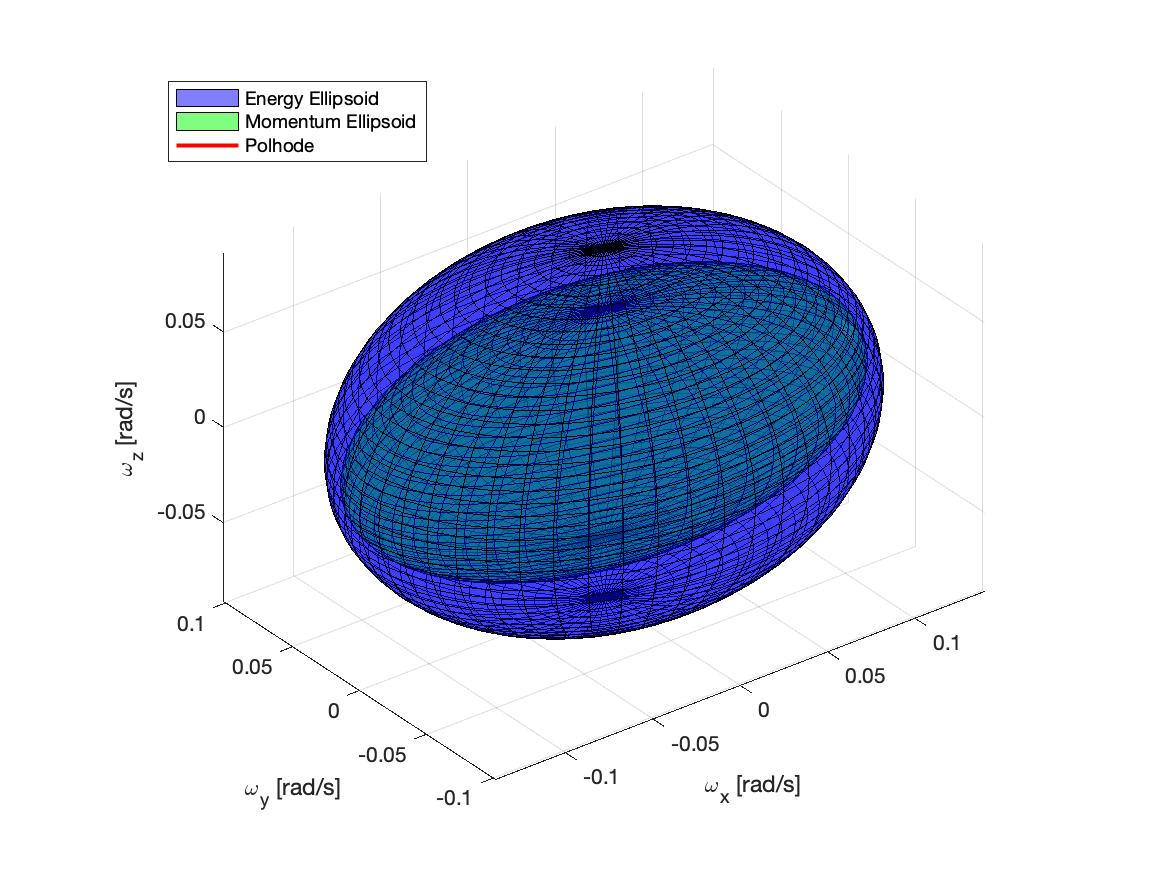
\includegraphics[scale=0.6]{Images/ps2_problem9_p7_x.png}
\caption{Polhode and ellipsoids for angular velocity vector for Case 1}
\label{fig:ps2_problem9_p7_x}
\end{figure}

\begin{figure}[H]
\centering
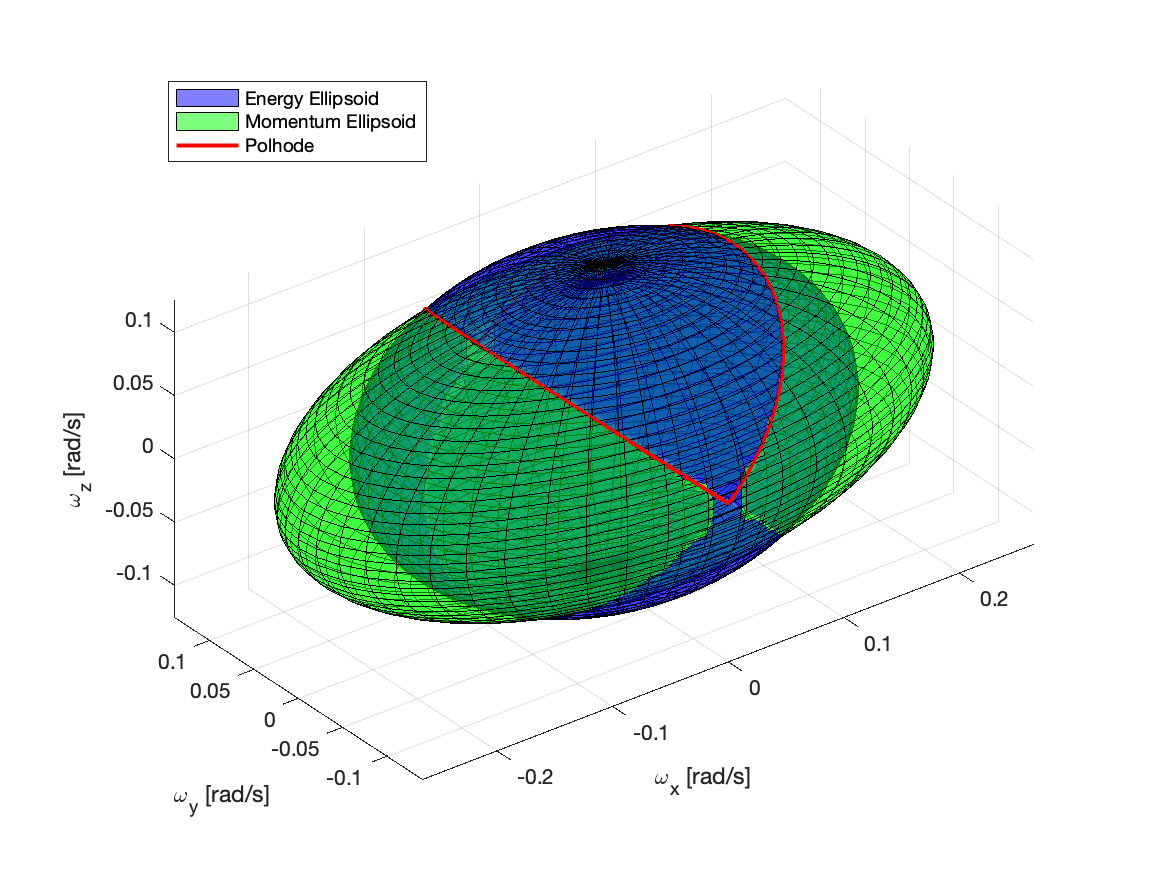
\includegraphics[scale=0.6]{Images/ps2_problem9_p7_y.png}
\caption{Polhode and ellipsoids for angular velocity vector for Case 2}
\label{fig:ps2_problem9_p7_y}
\end{figure}

\begin{figure}[H]
\centering
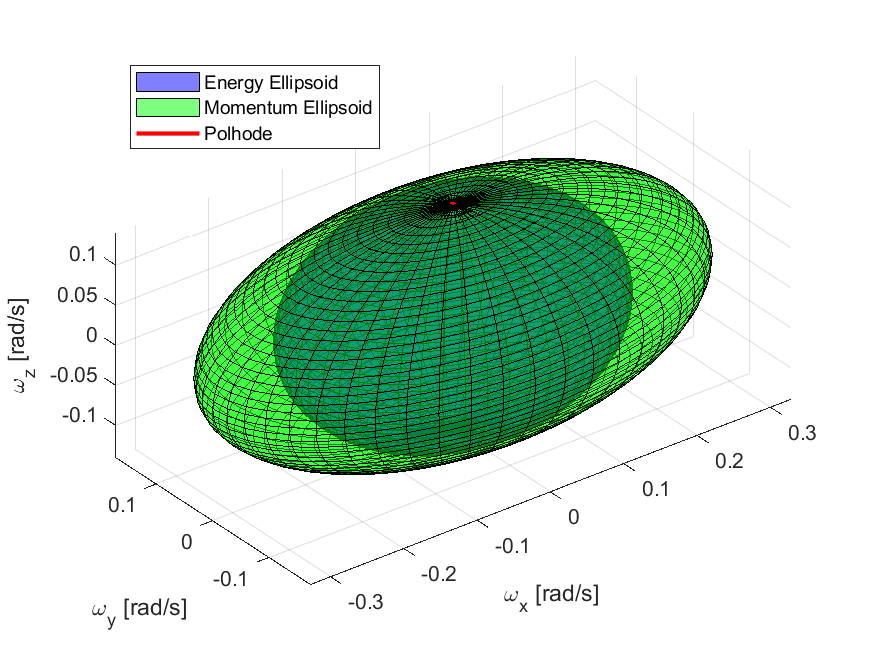
\includegraphics[scale=0.6]{Images/ps2_problem9_p7_z.png}
\caption{Polhode and ellipsoids for angular velocity vector for Case 3}
\label{fig:ps2_problem9_p7_z}
\end{figure}

\begin{figure}[H]
\centering
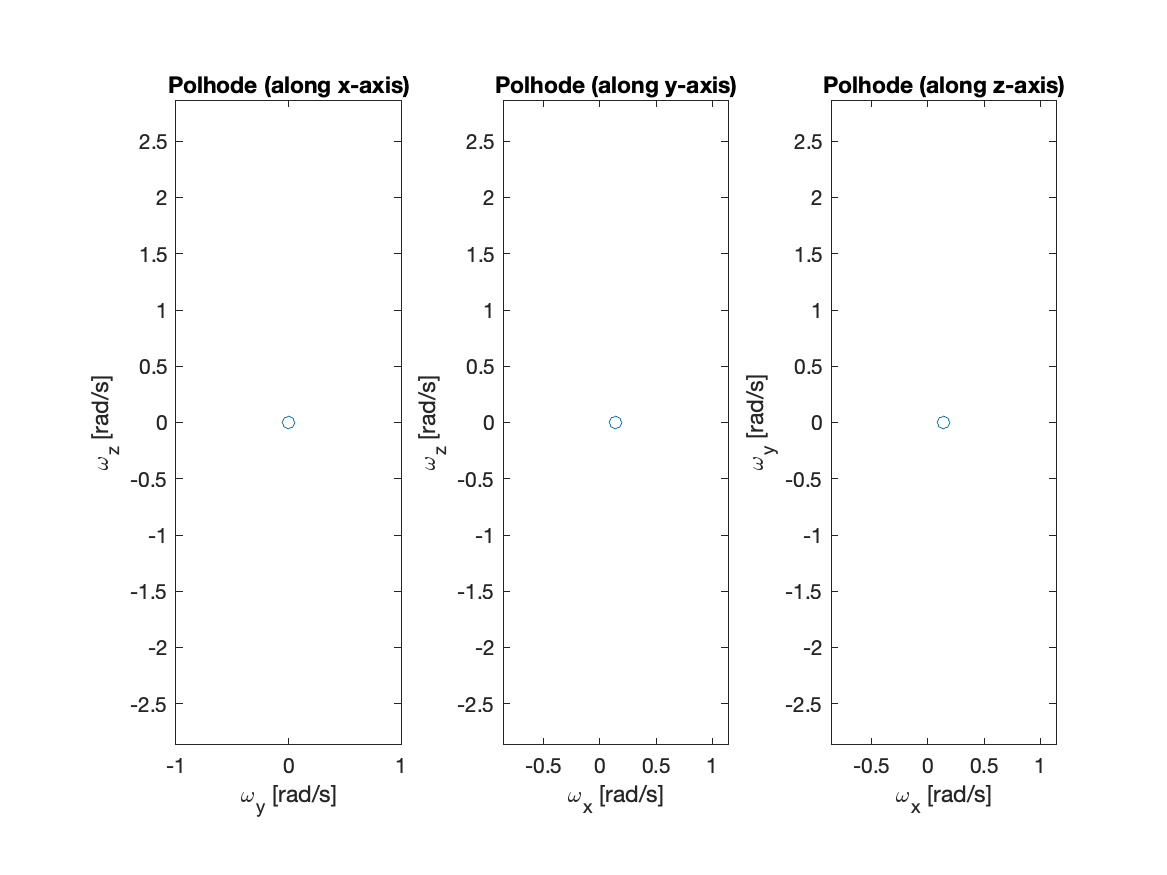
\includegraphics[scale=0.6]{Images/ps2_problem9_p8_x.png}
\caption{2D views of polhode for angular velocity vector for Case 1}
\label{fig:ps2_problem9_p8_x}
\end{figure}

\begin{figure}[H]
\centering
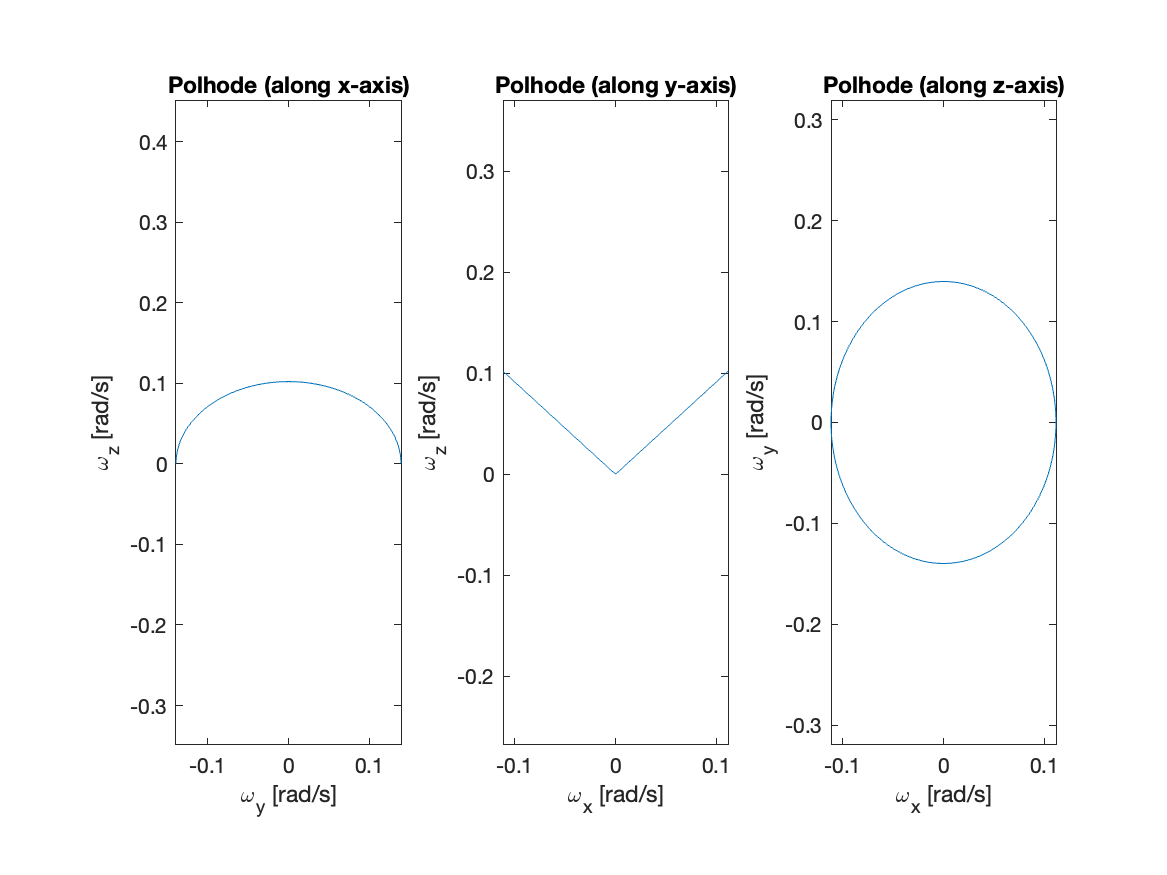
\includegraphics[scale=0.6]{Images/ps2_problem9_p8_y.png}
\caption{2D views of polhode for angular velocity vector for Case 2}
\label{fig:ps2_problem9_p8_y}
\end{figure}

\begin{figure}[H]
\centering
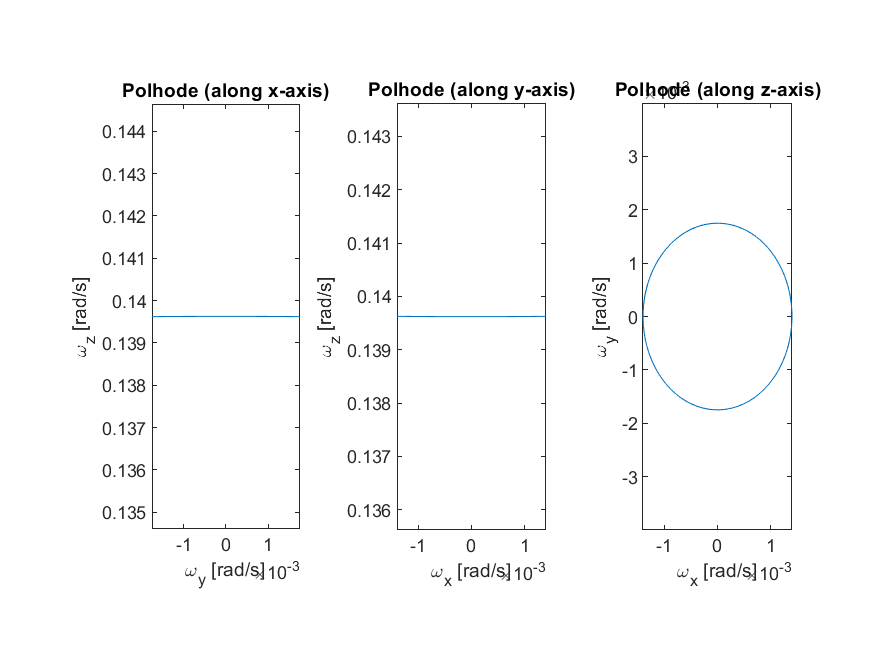
\includegraphics[scale=0.6]{Images/ps2_problem9_p8_z.png}
\caption{2D views of polhode for angular velocity vector for Case 3}
\label{fig:ps2_problem9_p8_z}
\end{figure}

\section{\Large PROBLEM SET 3}
\subsection{PROBLEM 1}
\textit{Impose that satellite is axial-symmetric (Ix$=$Iy$\neq$Iz). Repeat numerical simulation from previous pset using initial condition 4) from previous pset.}


\subsection{PROBLEM 2}
\textit{Program analytical solution for axial-symmetric satellite. Compute it at same time steps and from same initial conditions.}


\subsection{PROBLEM 3}
\textit{Compare numerical and analytical solutions. Plot differences (errors), do not only superimpose absolute values. Tune numerical integrator for large discrepancies. Are angular velocity vector and angular momentum vector changing according to theory in principal axes?}


\subsection{PROBLEM 4}
\textit{Program Kinematic equations of motion correspondent to a nominal attitude parameterization of your choice.}


\subsection{PROBLEM 5}
\textit{Program Kinematic equations of motion correspondent to a different attitude parameterization from the previous step. This is used for comparison, to get familiar with different approaches, and as fall back solution in the case of singularities.}


\subsection{PROBLEM 6}
\textit{Numerically integrate Euler AND Kinematic equations from arbitrary initial conditions (warning: stay far from singularity of adopted parameterization). Multiple revolutions. The output is the evolution of the attitude parameters over time. These attitude parameters describe orientation of principal axes relative to inertial axes.}


\subsection{PROBLEM 7}
\textit{ISince inertial position, velocity, and attitude, are known at the same time throughout the simulation, it is now possible to express vectors in the reference systems of interest.}



\section{\Large PROBLEM SET 4}
\subsection{PROBLEM 1}
\textit{Equilibrium tests}

\textit{a. Assume that 2 components of the initial angular velocities are zero and that the principal axes are aligned with the inertial frame (e.g., zero Euler angles). Verify that during the simulation the 2 components of angular velocity remain zero and that the attitude represents a pure rotation about the rotation axis (e.g., linearly increasing Euler angle). Plot velocities and angles.}

For this problem, we assumed that the initial angular velocity and Euler angles were what is shown below. The initial Euler angles were not initialized to be all 0 because we used 3-1-3 Euler angle representation, meaning that Euler angles at 0 would lead to a singularity. While this work-around is not ideal in the situation that the satellite operates around zero Euler angles, for the sake of this exercise this should be adequate.
\begin{align*}
\Vec{\omega} &= 
\qty[parse-numbers = false]{
    \begin{bmatrix}
    0 \\
    0 \\
    1 \\ 
    \end{bmatrix}
}{\radian\per\s}
\end{align*}
\begin{align*}
\phi = \qty[parse-numbers = false]{0}{\radian}, \;\;\;
\theta = \qty[parse-numbers = false]{1e-9}{\radian}, \;\;\;
\psi = \qty[parse-numbers = false]{0}{\radian}
\end{align*}

As can be seen in Figure \ref{fig:ps4_problem1a_velocity}, $\omega_x$ and $\omega_y$ remained 0, while $\omega_z$ was a constant value, as expected. Similarly, in Figure \ref{fig:ps4_problem1a_angle} the $\phi$ and $\theta$ Euler angles stayed zero while the $\psi$ Euler angle varied. 

\begin{figure}[H]
\centering
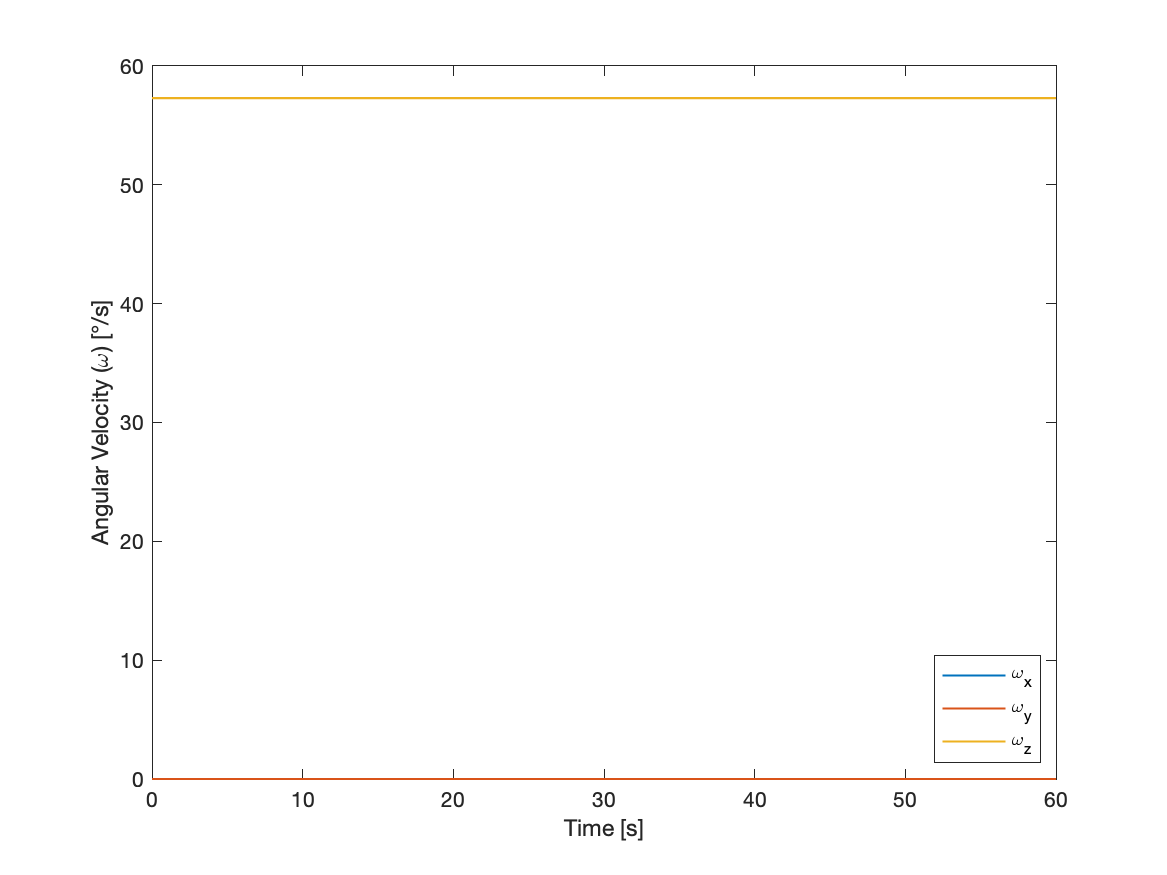
\includegraphics[scale=0.6]{Images/ps4_problem1a_angvel.png}
\caption{Evolution of angular velocity}
\label{fig:ps4_problem1a_angvel}
\end{figure}

\begin{figure}[H]
\centering
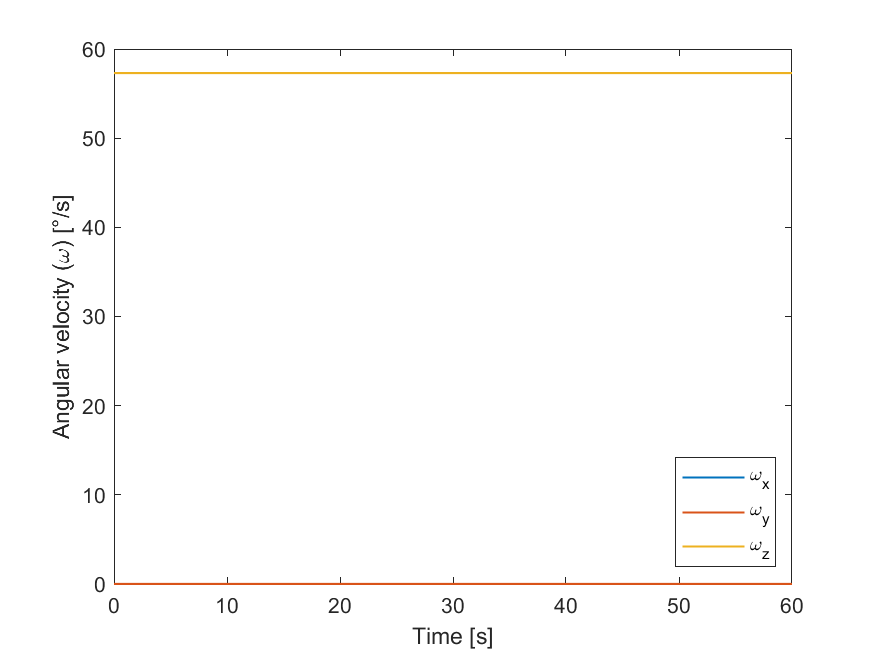
\includegraphics[scale=0.6]{Images/ps4_problem1a_angle.png}
\caption{Evolution of Euler angles}
\label{fig:ps4_problem1a_angle}
\end{figure}

\textit{b. Repeat a. by setting the initial attitude to match the RTN frame. Set the initial angular velocity to be non-zero only about N. Show the evolution of attitude motion in the RTN frame and give an interpretation of the results (recall that you might have J2 effects in orbit propagation, consider removing them for verification).}

In the event that initial angular velocity is along only the normal, the angular velocity remains constant throughout the orbit, as seen in Figure \ref{fig:ps4_problem1b_angvel}. From Figure \ref{fig:ps4_problem1b_euler}, we see that the $\theta$ and $\psi$ Euler angles are constant while $\phi$ varies.

\begin{figure}[H]
\centering
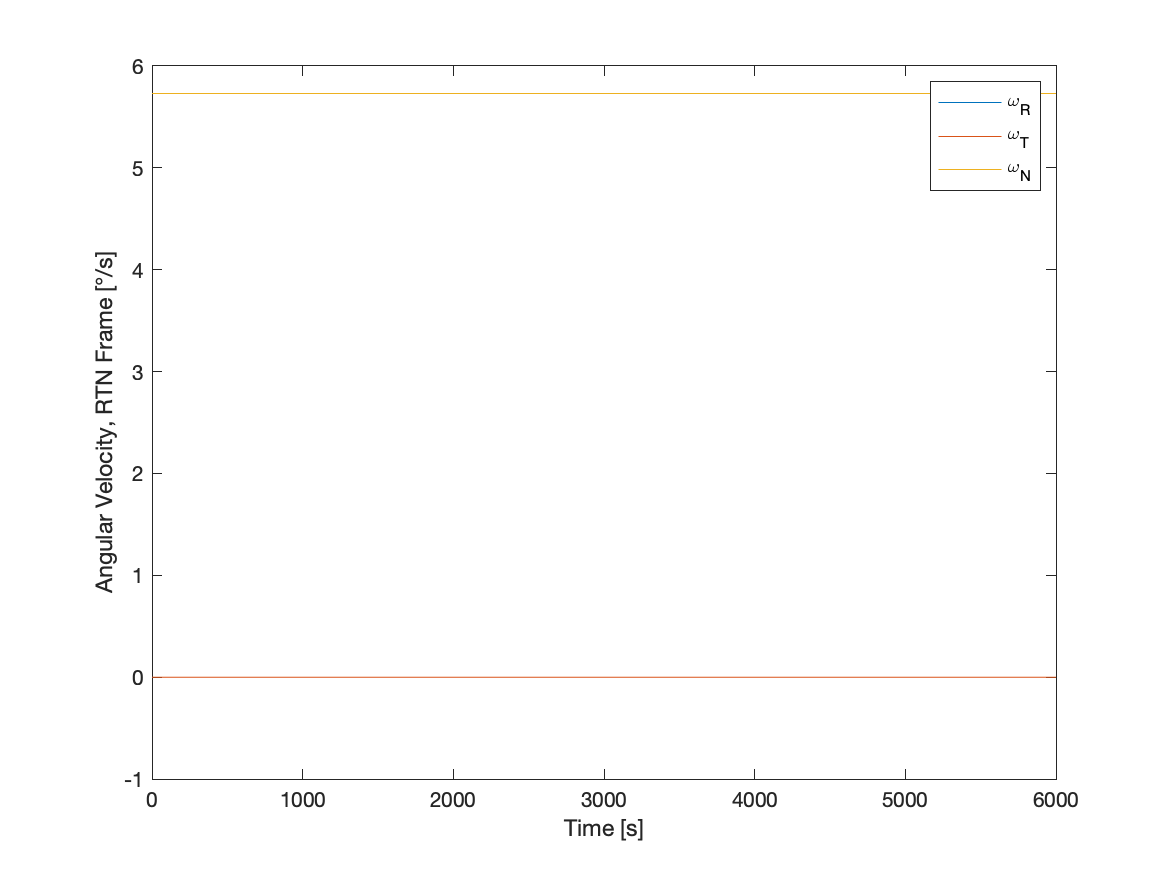
\includegraphics[scale=0.6]{Images/ps4_problem1b_angvel.png}
\caption{Evolution of angular velocity}
\label{fig:ps4_problem1b_angvel}
\end{figure}

\begin{figure}[H]
\centering
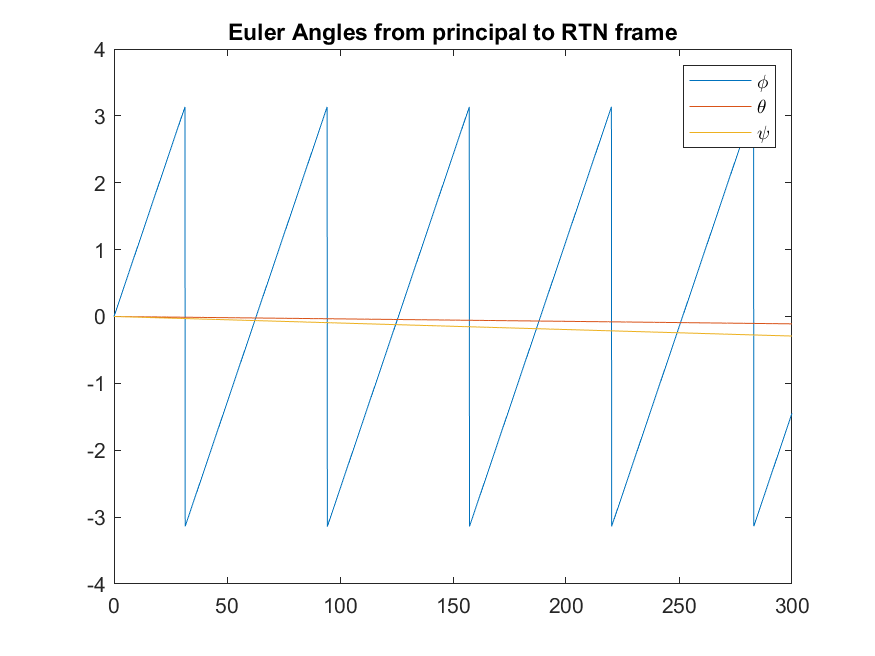
\includegraphics[scale=0.6]{Images/ps4_problem1b_euler.png}
\caption{Evolution of Euler angles}
\label{fig:ps4_problem1b_euler}
\end{figure}


\subsection{PROBLEM 2}
\textit{Stability tests}

\textit{a. Pretend you have a single-spin satellite. Set initial conditions to correspond alternatively to the 3 possible equilibrium configurations (rotation about principal axes of inertia). Slightly perturb initial condition. Is the attitude stable or unstable? In angles and velocities? If stable, periodically or asymptotically? Show it.}

For a single spin satellite, the three possible equilibrium configurations are spinning on its minimum principal axis, spinning on its intermediate principal axis, and spinning on its
maximum principal axis. Figures \ref{fig:ps4_problem2a_1}, \ref{fig:ps4_problem2a_2}, \ref{fig:ps4_problem2a_3}, all show that the Euler angles are relatively unstable in for the intermediate and minimum axes, and is much more stable along the maximum axis. However, the angular velocities are periodically stable when spinning along the minimum and maximum axes and unstable when spinning on the intermediate axis.

\begin{figure}[H]
\centering
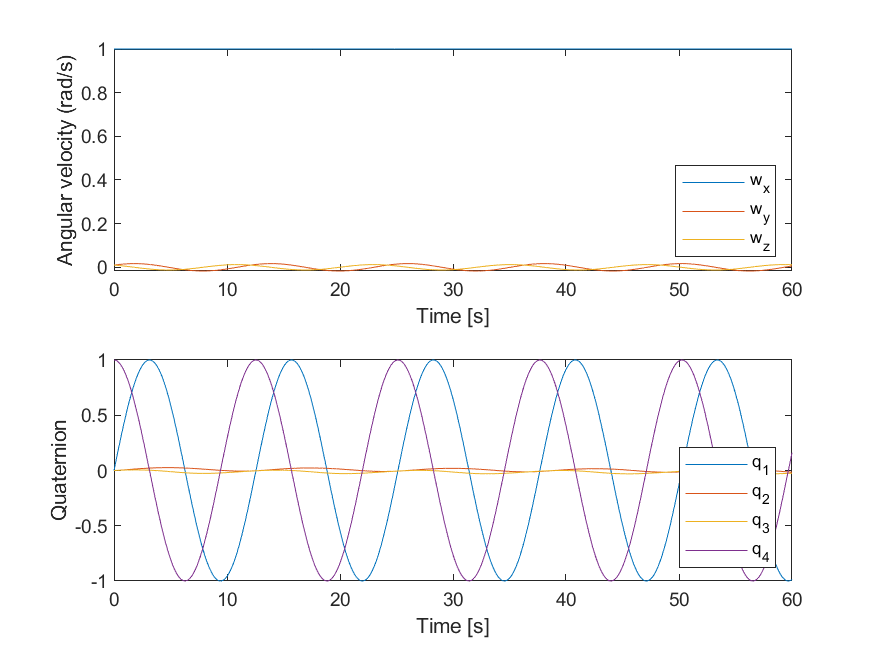
\includegraphics[scale=0.6]{Images/ps4_problem2a_1.png}
\caption{Simulation of satellite spinning on its minimum principal axis}
\label{fig:ps4_problem2a_1}
\end{figure}

\begin{figure}[H]
\centering
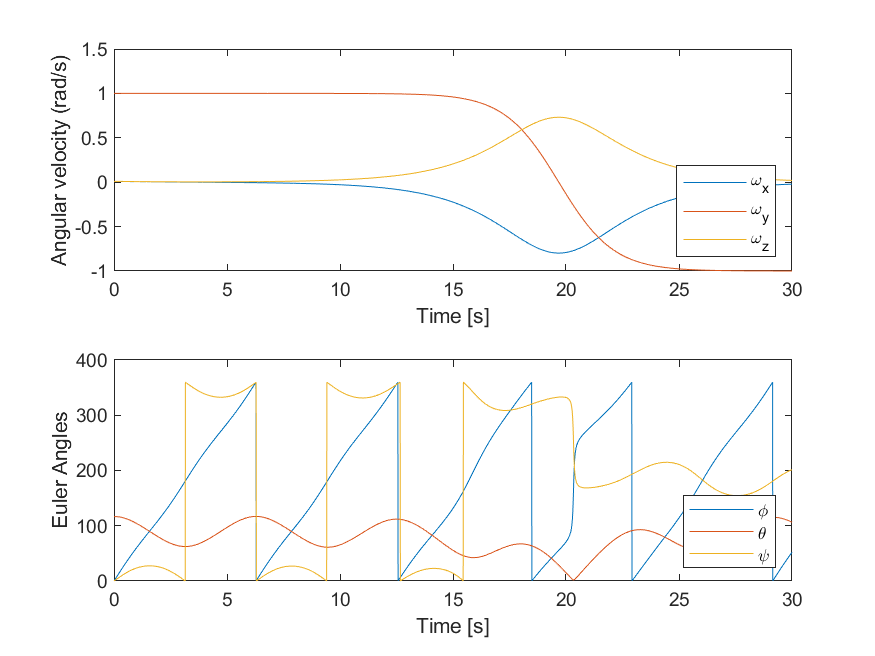
\includegraphics[scale=0.6]{Images/ps4_problem2a_2.png}
\caption{Simulation of satellite spinning on its intermediate principal axis}
\label{fig:ps4_problem2a_2}
\end{figure}

\begin{figure}[H]
\centering
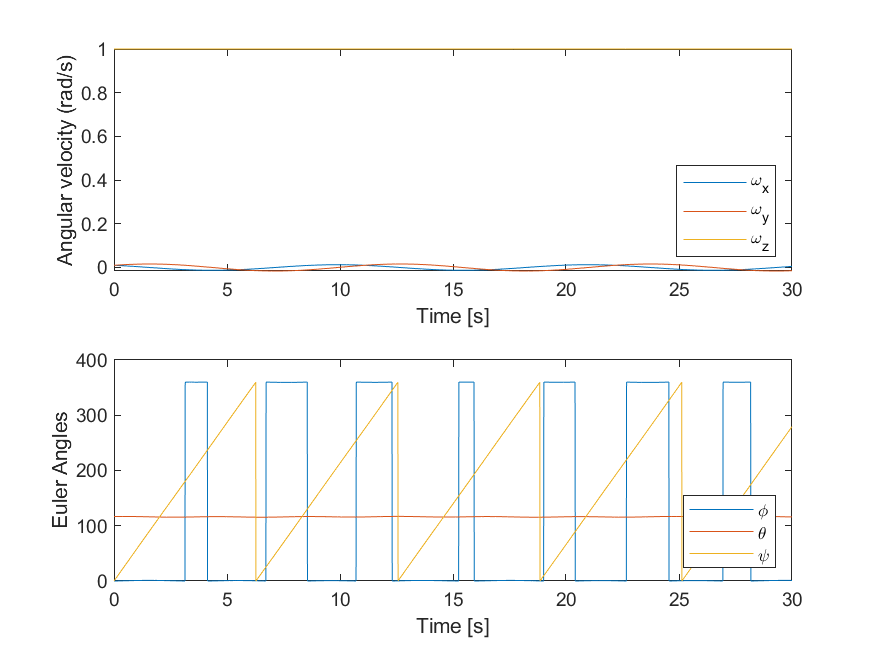
\includegraphics[scale=0.6]{Images/ps4_problem2a_3.png}
\caption{Simulation of satellite spinning on its maximum principal axis}
\label{fig:ps4_problem2a_3}
\end{figure}

\subsection{PROBLEM 3}
\textit{Adding a momentum wheel or rotor (dual-spin satellite)}

\textit{a. Re-program Euler equations to include a generic momentum wheel or rotor with rotation axis aligned with one of the principal axes of inertia. Ideally the wheel or rotor has specs representative of commercial products (inertia, rotational speed).}

The equations that implement the generic momentum wheel with the rotor into the Euler equations are below.

\begin{align*}
    I_x \dot{\omega_x} + I_r \dot{\omega_r} r_x + (I_z - I_y) \omega_y \omega_z 
    + I_r \omega_r (\omega_y r_z - \omega_z r_y) = M_x \\
    I_y \dot{\omega_y} + I_r \dot{\omega_r} r_y + (I_x - I_z) \omega_z \omega_x 
    + I_r \omega_r (\omega_z r_x - \omega_x r_z) = M_y \\
    I_z \dot{\omega_z} + I_r \dot{\omega_r} r_z + (I_y - I_x) \omega_x \omega_y 
    + I_r \omega_r (\omega_x r_y - \omega_y r_x) = M_z \\
    I_r \dot{\omega_r} = M_r
\end{align*}

The function kinEulerAngleWheel was used in addition to ode113 to simulate the angular velocities over time.

\textit{b. Numerically integrate Euler AND Kinematic equations from equilibrium initial condition. Verify that integration is correct as from previous tests (conservation laws, rotations, etc.).}

kinEulerAngleWheel was modified to also account for the kinematic equations, as shown before. As we see in Figure \ref{fig:ps4_problem3c_principal}, the overall momentum is conserved in the principal frame, as expected. Additionally, Figure \ref{fig:ps4_problem3c_inertial} shows that the angular momentum vector is conserved in the inertial frame, as expected.

\lstinputlisting{src/kinEulerAngleWheel.m}

\begin{figure}[H]
\centering
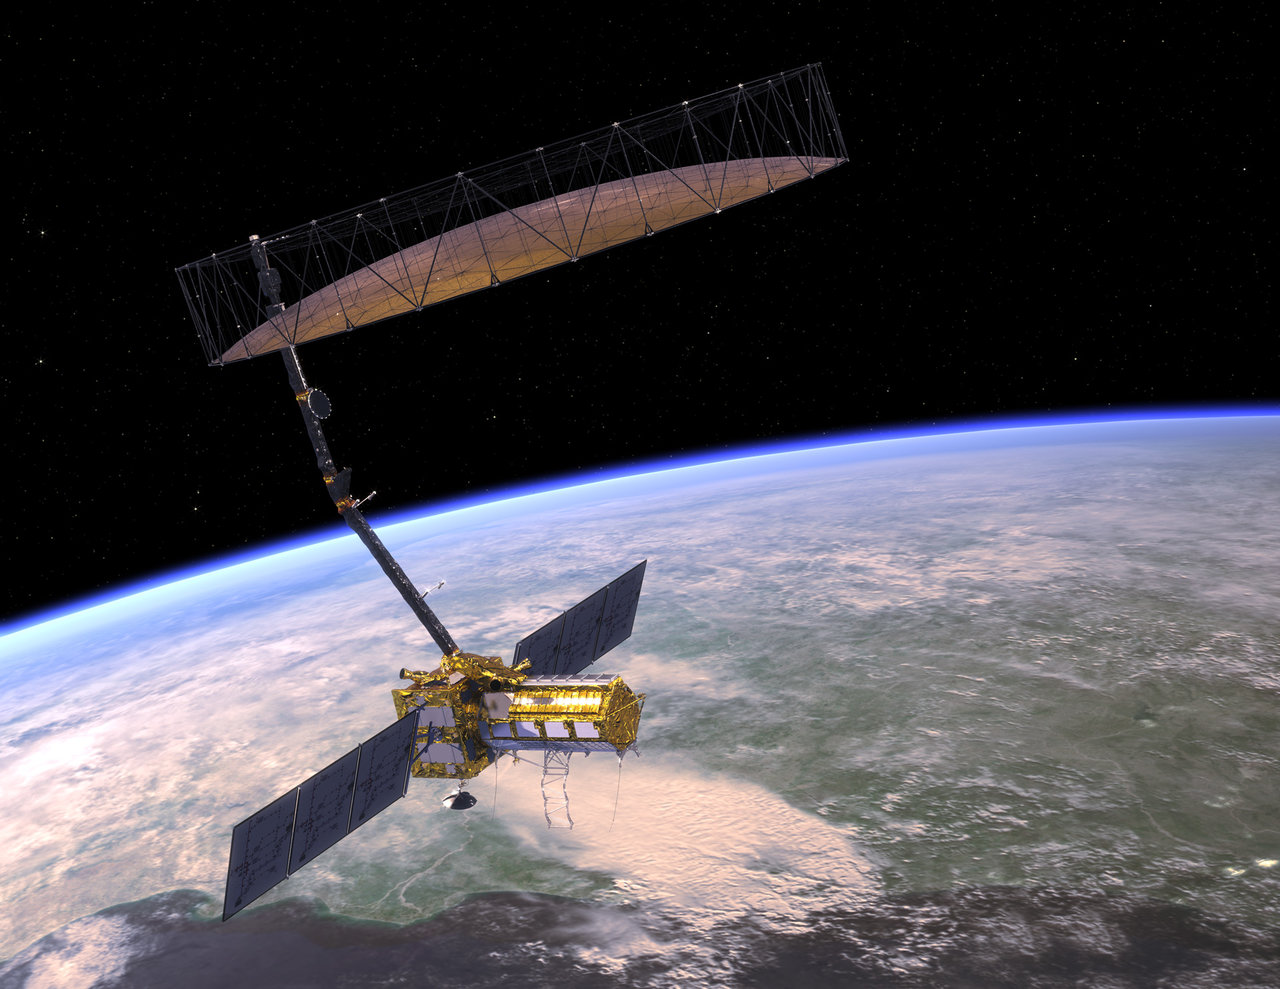
\includegraphics[scale=0.6]{Images/NISAR.jpg}
\caption{Angular Momentum in Principal Frame}
\label{fig:ps4_problem3c_principal}
\end{figure}

\begin{figure}[H]
\centering
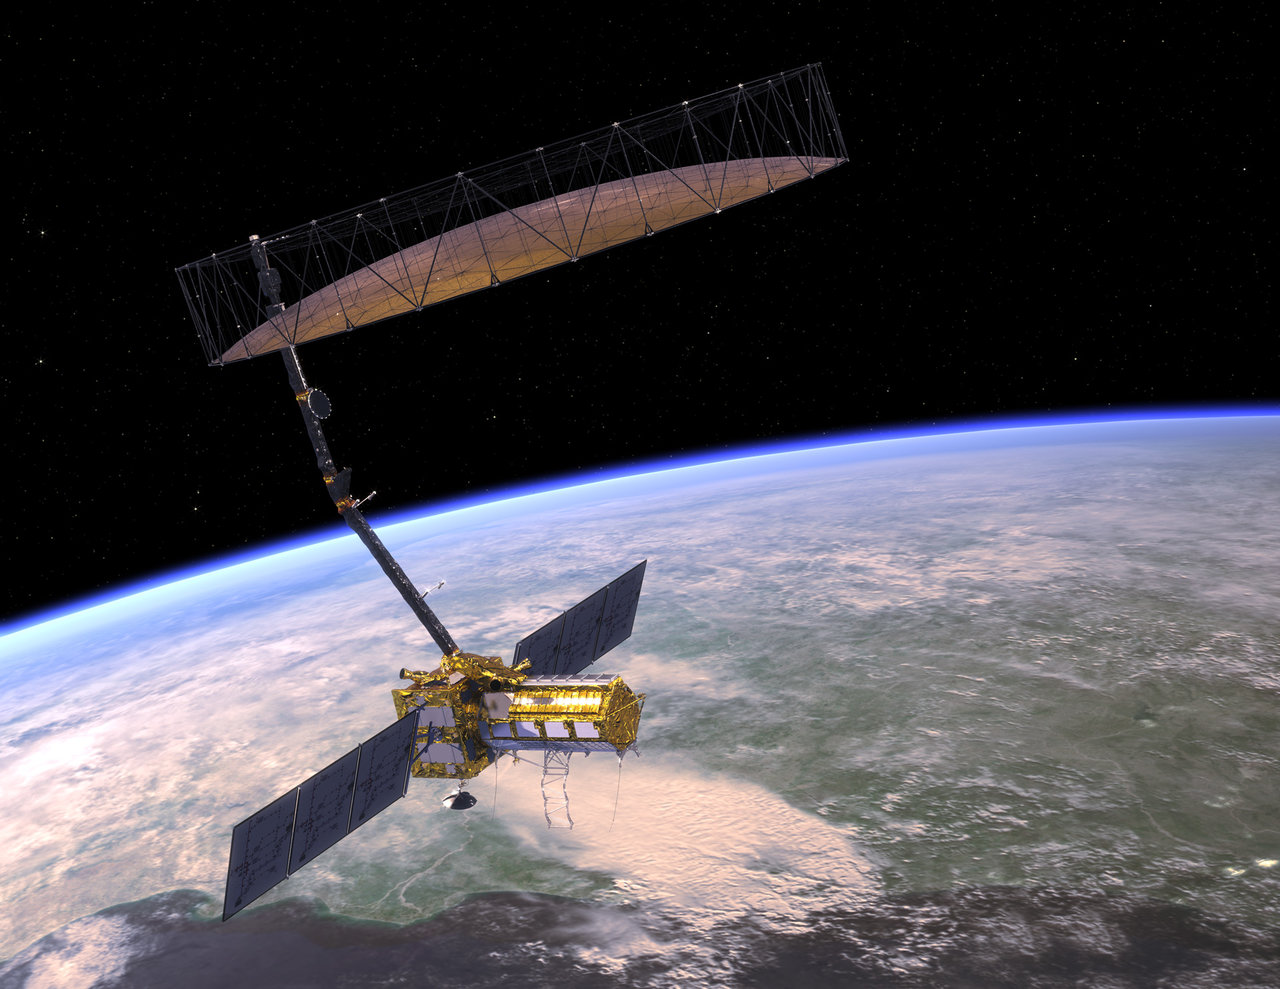
\includegraphics[scale=0.6]{Images/NISAR.jpg}
\caption{Angular Momentum in Inertial Frame}
\label{fig:ps4_problem3c_inertial}
\end{figure}

\textit{c. Verify equilibrium and its stability similar to previous pset.}

Based on linearizing the Euler equations around equilibrium, it can be found that periodic stability can be met with a reaction wheel if one of the following conditions are met:

\begin{align*}
    1)\; I_r \omega_r > (I_y - I_z) \omega_z \;\; AND \;\; I_r \omega_r > (I_x - I_z) \omega_z \\
    2)\; I_r \omega_r < (I_y - I_z) \omega_z \;\; AND \;\; I_r \omega_r < (I_x - I_z) \omega_z \\
\end{align*}

The above equation is specifically for equilibrium about the z-axis, but similar equations hold true for stability about the x and y axes.

Below are the angular velocity plots for stability about the maximum, intermediate, and minimum principal axes.

\textbf{figs}


\textit{d. Use the stability condition to make attitude motion stable for rotation about intermediate moment of inertia by changing moment of inertia and/or angular velocity of the momentum wheel or rotor.}




\textit{e. Try to make rotation about another arbitrary axis (potentially relevant to your project) stable through a generic momentum wheel or rotor.}

\subsection{PROBLEM 4}
\textit{Gravity gradient torque (modeling)}

\textit{a. Remove rotor.}

A new function was created without effect of the rotor.

\textit{b. Program gravity gradient torque. Feed torque to Euler equations. This is the first perturbation you model resulting from the interaction of the spacecraft with the environment. Hint: change your orbit to make gravity gradient significant if that’s not the case.}

The equations for the gravity gradient torque are below.

\begin{align*}
    I_x \dot{\omega_x} + (I_z - I_y) \omega_y \omega_z = 3 n^2 (I_z - I_y) c_y c_z \\
    I_y \dot{\omega_y} + (I_x - I_z) \omega_z \omega_x = 3 n^2 (I_x - I_z) c_z c_x \\
    I_z \dot{\omega_z} + (I_y - I_x) \omega_x \omega_y = 3 n^2 (I_y - I_x) c_x c_y \\
\end{align*}

In the above equation, $\Vec{c} = [cx, cy, cz]$ is the normalized direction of $\Vec{R}$.

The function gravGrad was developed to be used with ode113 to propagate the Euler equations.

\lstinputlisting{src/gravGrad.m}

\textit{c. Verify that the magnitude of the modeled torque is consistent with the orbit and inertia tensor of your satellite. Hint: use simplified formulas from class on modeling of gravity gradient torque.}

The general trends we would expect in the gradient gravity torque is for the value to be zero if the satellite spins on its normal axis at the mean motion and for the magnitude to grow linearly with the inertia tensor. The first property is demonstrated in Figure \textbf{fig1} and the second is demonstrated in Figure \textbf{fig2}.

Additionally, we can estimate the order of magnitude to expect our gravity gradient torques to be based on the below equation.

\begin{align*}
    \Vec{M} &= \frac{3 \mu}{a^3}
    \begin{bmatrix}
    (I_z - I_y) c_y c_z \\
    (I_x - I_z) c_z c_x \\
    (I_y - I_x) c_x c_y
    \end{bmatrix}
\end{align*}

The parameters used were the known moments of inertia ($I_x = \qty{7707}{}$, $I_y = \qty{14563}{}$, $I_z = \qty{18050}{\kilogram\cdot\meter^2}$), known values for Earth ($a = \qty{7125.49}{km}$, $\mu = \qty{398600}{\km^3\per\second^2}$), and an arbitrary $\Vec{c} = [\frac{1}{\sqrt{3}}, \frac{1}{\sqrt{3}}, \frac{1}{\sqrt{3}}]$. With these values, we get:

\begin{align*}
    \Vec{M} &=
\qty[parse-numbers = false]{
    \begin{bmatrix}
    0.384174 \\
    1.13956 \\
    -0.755387
    \end{bmatrix}
    \cdot
    10^{-2}
}{\newton\meter}
\end{align*}

These values are in line with what we see in Figure \textbf{fig}.

\textit{d. Numerically integrate Euler and Kinematic equations including gravity gradient from initial conditions corresponding to body axes aligned with the orbital frame (RTN). Verify that gravity gradient torque is zero, besides numerical errors. Hint: you may need to simplify the orbit to unperturbed circular to achieve this. Check that initial angular velocity matches mean motion.}

The constant gravity gradient was demonstrated in problem 4c in Figure \textbf{same fig as before}. Figure \textbf{fig3} demonstrated that the angular velocity in the normal direction matches the mean motion throughout the orbit.

\textit{e. Numerically integrate Euler and Kinematic equations including gravity gradient from arbitrary initial conditions (e.g., relevant to your project). Plot external torque (3 components w.r.t. time) and resulting attitude motion (depends on attitude parameterization, add Euler angles for better geometrical interpretation) over multiple orbits. Comment on results.}

fuck me with a shoe idk what to put here rn (will add later)

\section{\Large PROBLEM SET 5}
\subsection{PROBLEM 1}
\textit{Gravity gradient torque (stability)}

\textit{a. Calculate the coefficients Ki of the moments of inertia which drive stability under gravity gradient. Compute and plot regions of stable and unstable motion similar to the picture below:}

The following equations show the relationships for gravity gradient stability in terms of moments of inertia. The first inequality hold for when the pitch is stable, and the last two inequalites hold for when the roll and yaw are stable.

\begin{align*}
    k_N = \frac{I_T - I_R}{I_N}, \;\;\;\;\;
    k_T = \frac{I_N - I_R}{I_T}, \;\;\;\;\;
    k_R = \frac{I_N - I_T}{I_R} \\
    k_T > k_R, \;\;\;\;\;
    k_R k_T > 0, \;\;\;\;\;
    1 + 3 k_T + k_R k_T > 4 \sqrt{k_R k_T}
\end{align*}

We show the plot of stable and unstable motion under gravity gradient. When computing the coefficients using moments of inertia about the principal axes, we obtain the following plot. In this case, we investigate the stability for the satellite when it is rotated such that the spacecraft is oriented appropriately for SAR operations, that is, principal x-axis is anti-radial, principal y-axis is opposite of cross-track, and principal z-axis is opposite of along-track. However, this orientation is unstable, as shown below.

\begin{figure}[H]
\centering
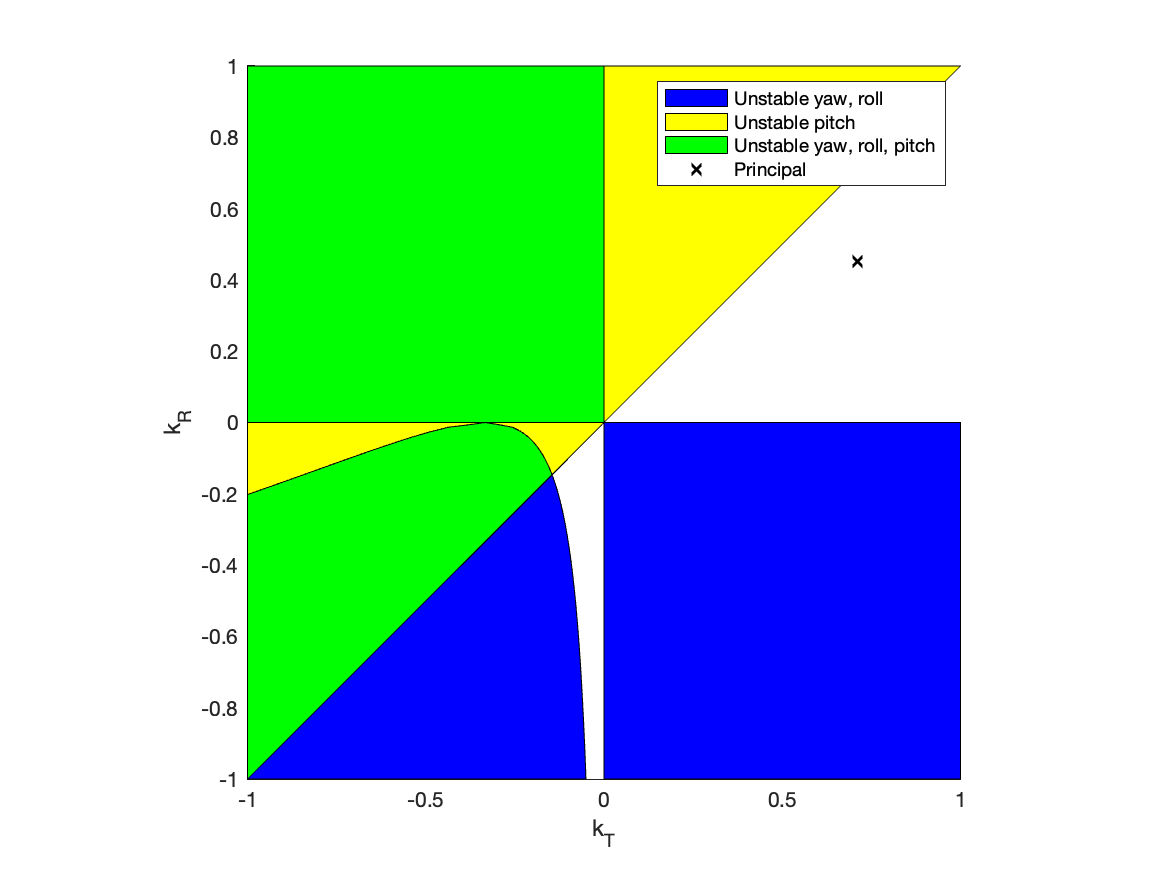
\includegraphics[scale=0.8]{Images/ps5_problem1a.png}
\caption{Stability for nominal axes}
\label{fig:ps5_problem1a}
\end{figure}

\textit{b. Considering the results from 1a, comments on the expected stability of the attitude motion of your satellite about equilibrium. Try to reproduce stable and unstable motion by setting proper initial conditions and perturbing those conditions slightly (e.g., by 1\%). Plot attitude parameters (e.g., Euler angles) to show stability or instability.}

First, without perturbations, the satellite can maintain steady attitude, demonstrating that this chosen orientation is indeed an equilibrium.

\begin{figure}[H]
\centering
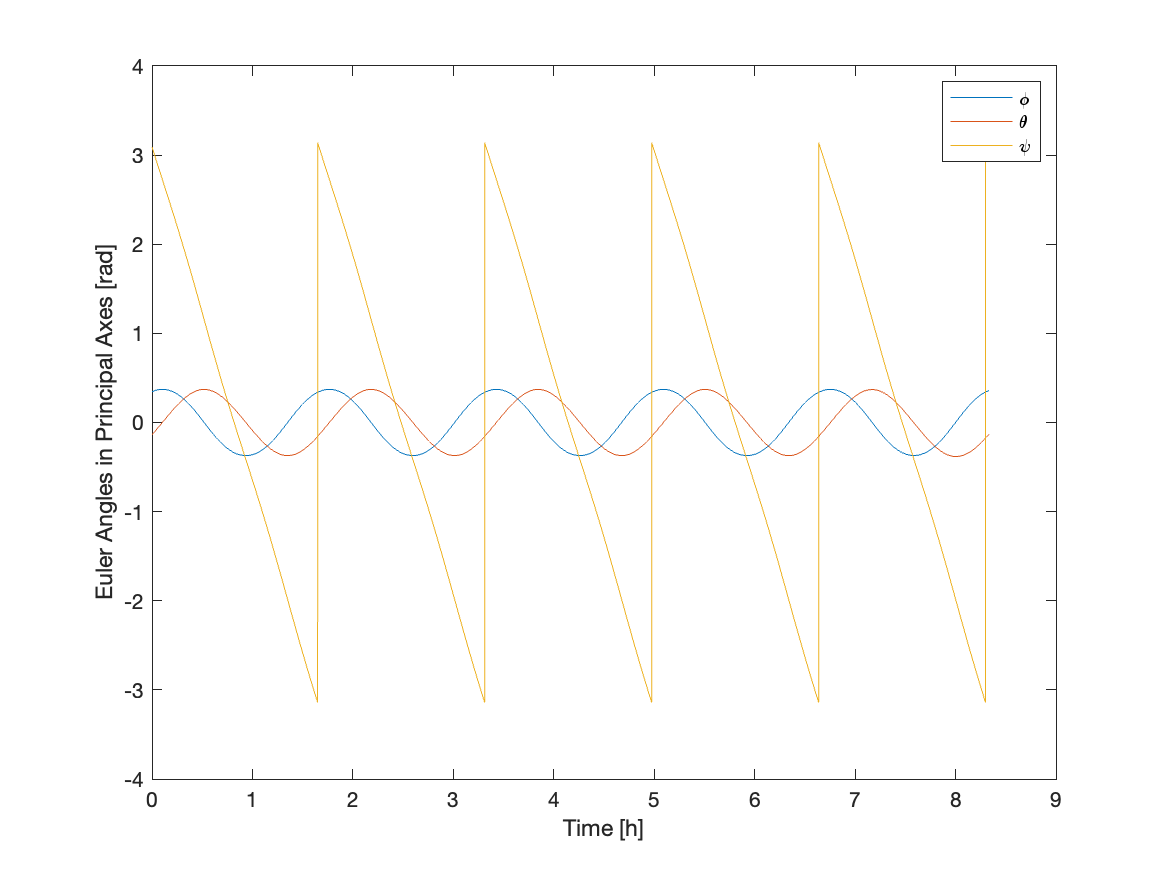
\includegraphics[scale=0.6]{Images/ps5_problem1b_angle_unperturbed.png}
\caption{Attitude evolution for unstable orientation without perturbations}
\label{fig:ps5_problem1b_angle_unperturbed}
\end{figure}

\begin{figure}[H]
\centering
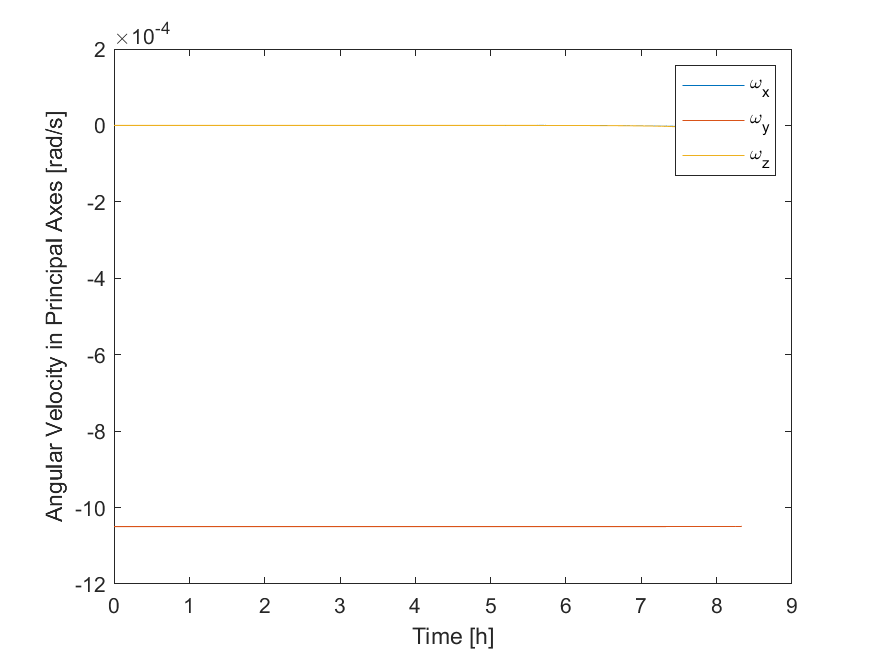
\includegraphics[scale=0.6]{Images/ps5_problem1b_angvel_unperturbed.png}
\caption{Angular velocity evolution for unstable orientation without perturbations}
\label{fig:ps5_problem1b_angvel_unperturbed}
\end{figure}

We expect unstable behavior for small perturbations. Previously, we have already shown that aligning principal axes with RTN produces stable behavior when there are no perturbations. Now, we will introduce small perturbations, causing the system to leave equilibrium and demonstrating that it is unstable.

\begin{figure}[H]
\centering
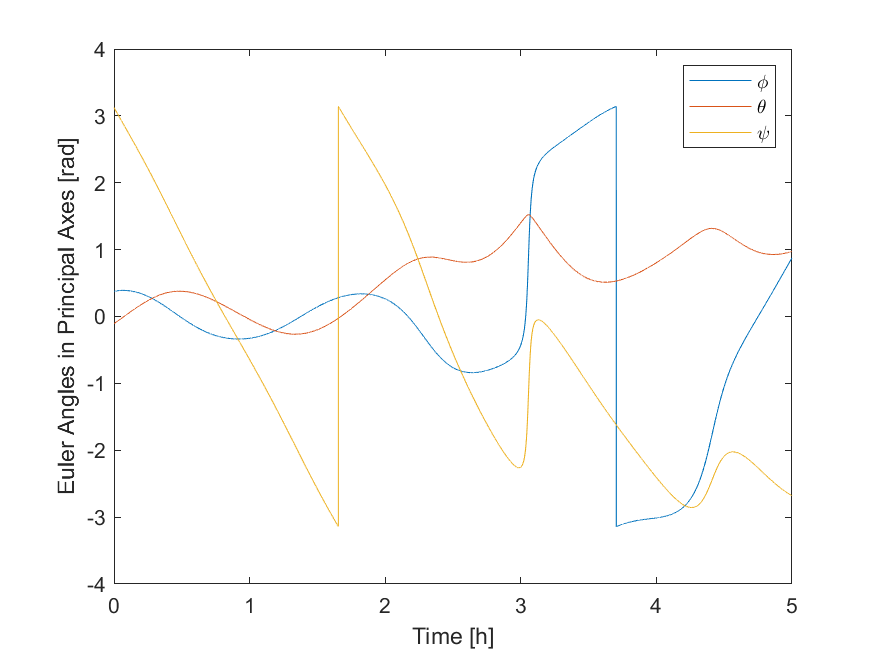
\includegraphics[scale=0.6]{Images/ps5_problem1b_angle.png}
\caption{Attitude evolution for unstable orientation with 1\% perturbations}
\label{fig:ps5_problem1b_angle}
\end{figure}

\begin{figure}[H]
\centering
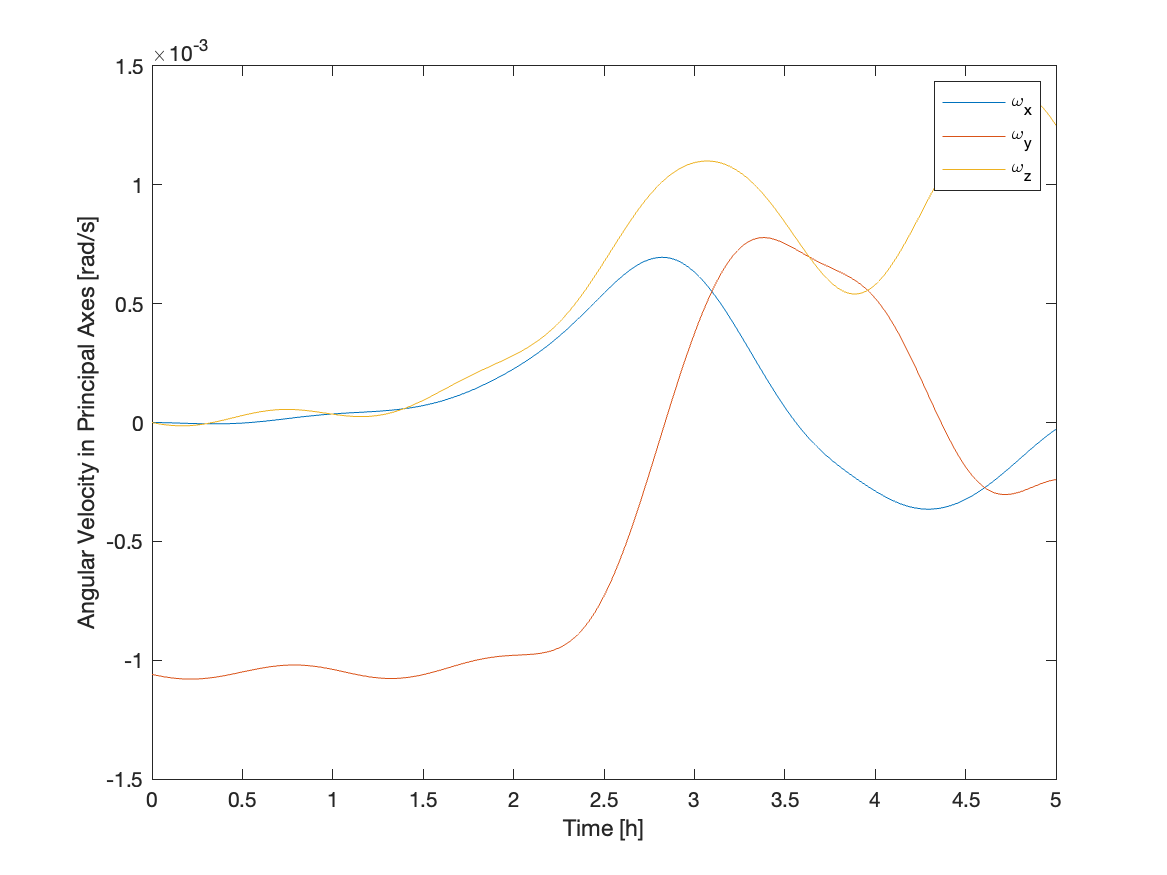
\includegraphics[scale=0.6]{Images/ps5_problem1b_angvel.png}
\caption{Angular velocity evolution for unstable orientation with 1\% perturbations}
\label{fig:ps5_problem1b_angvel}
\end{figure}


\textit{c. How would you need to change the mass distribution and/or nominal attitude of your satellite to obtain stable motion from the gravity gradient torque? Would it make sense for your project? Show a couple of potential configurations in the Ki plane and resulting stability of attitude motion at the equilibrium. This is done by changing your inertia tensor and simulating numerically.}

We will have to align the principal axes XYZ with RTN (respectively) to obtain a stable attitude motion.

\begin{figure}[H]
\centering
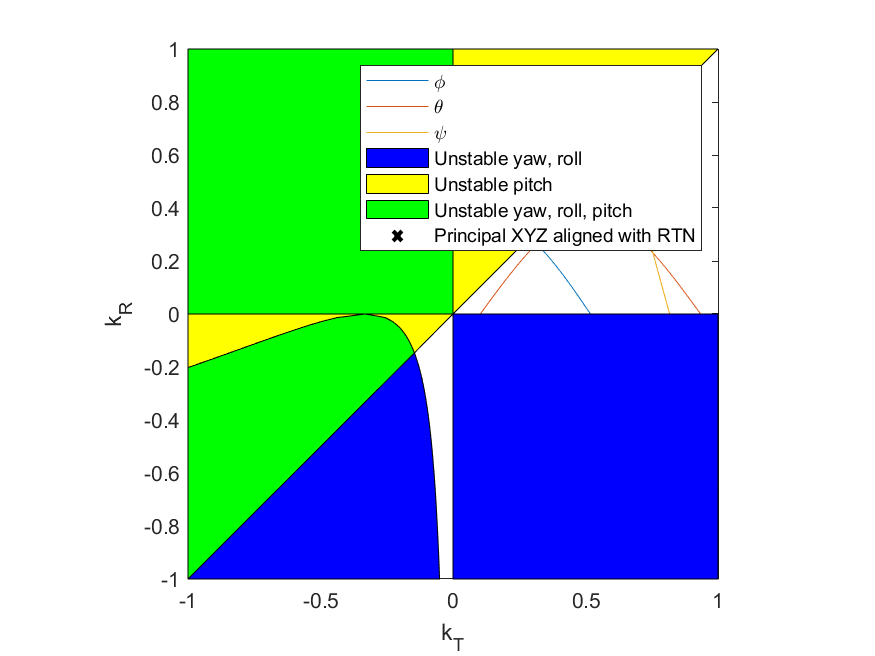
\includegraphics[scale=0.8]{Images/ps5_problem1c.png}
\caption{Stability for aligned principal axes}
\label{fig:ps5_problem1c}
\end{figure}

We expect stable behavior for small perturbations. Previously, we have already shown that aligning principal axes with RTN produces stable behavior when there are no perturbations. Now, we will introduce small perturbations.

\begin{figure}[H]
\centering
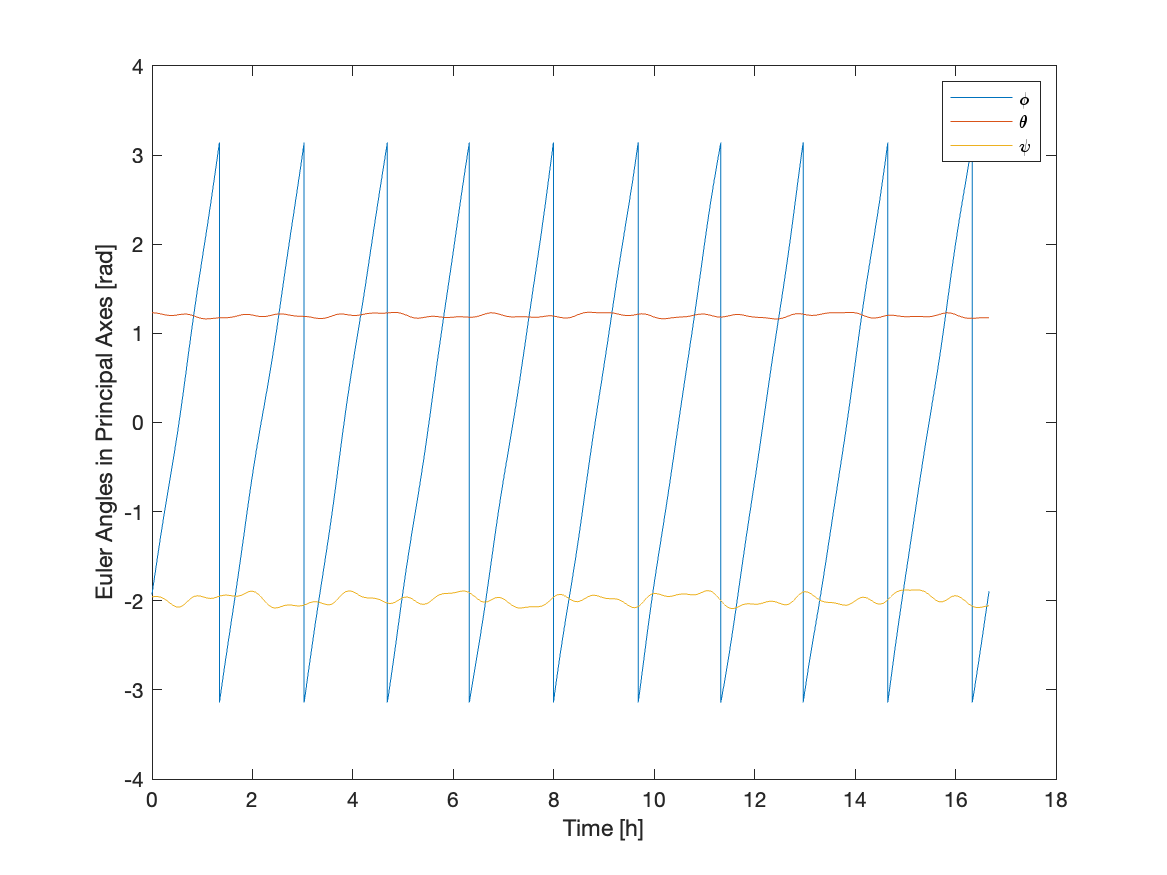
\includegraphics[scale=0.6]{Images/ps5_problem1c_angle.png}
\caption{Attitude evolution for stable orientation with 1\% perturbations}
\label{fig:ps5_problem1c_angle}
\end{figure}

\begin{figure}[H]
\centering
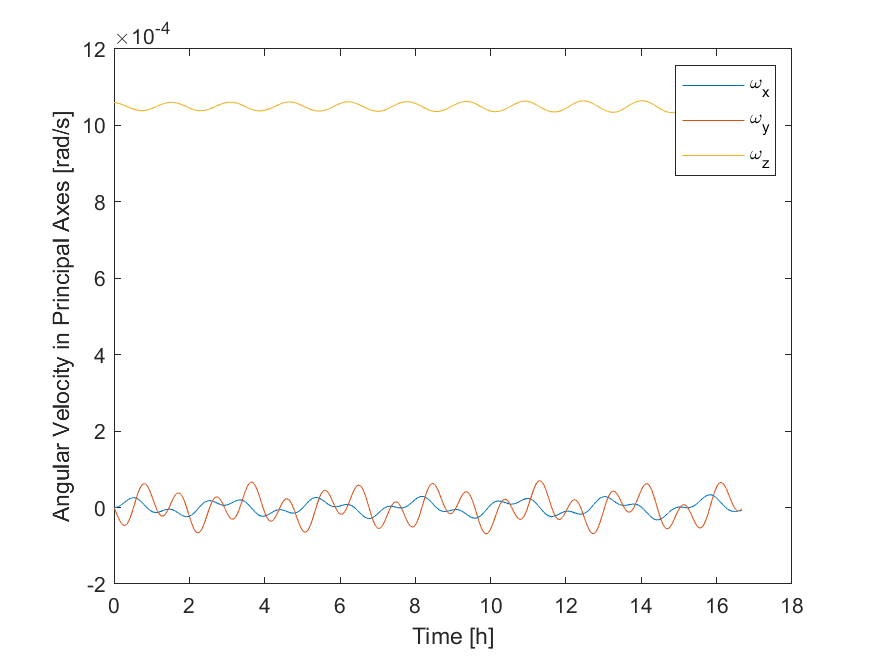
\includegraphics[scale=0.6]{Images/ps5_problem1c_angvel.png}
\caption{Angular velocity evolution for stable orientation with 1\% perturbations}
\label{fig:ps5_problem1c_angvel}
\end{figure}

As expected, our attitude motion (angular velocities and Euler angles) are periodically stable with a small perturbation in initial condition.

We cannot maintain this orientation if we want to properly point the radar antenna located at the top of the spacecraft, so it does not make sense to orient the satellite along principal axes for gravity gradient stability. Instead, we will likely require magnetorquers to offset angular momentum changes from environmental torques, including gravity gradient torques due to our unstable equilibrium.


\subsection{PROBLEM 2}
\textit{In addition to gravity gradient, start programming perturbation torques due to magnetic field, solar radiation pressure, and atmospheric drag. Note 1: You should apply a very minimal/basic model for perturbations that are not relevant (negligible) to your project. It is expected that you do not ignore them. Note 2: All perturbations can be grouped into a single large subsystem called environment or similar whose output feed
the Euler equations. Note 3: Re-use as many functions as possible for solar radiation pressure and atmospheric drag.}

In addition to gravity gradient torques, we modeled torque from magnetic field interactions, solar radiation pressure, and atmospheric drag.

The equation for the torque from the magnetic field interactions is shown below.

\begin{align*}
    \Vec{M}_{m} = \Vec{m}_{sat} \times \Vec{B}_{Earth}
\end{align*}

Since the satellite is operates in LEO, the spherical harmonic model up to n = 4 was used for maximum accuracy. This model is based on the geocentric distance ($R$), colatitude ($\theta$), and longitude ($\phi$). The model requires Gaussian coefficients ($g^{n,m}$, $h^{n,m}$) and Legendre functions ($P^{n,m}$) and their derivatives ($\frac{\delta P^{n,m} (\theta)}{\delta \theta}$), which are explained in more detail in Wertz \cite{Wertz}.

\begin{align*}
    B_R = \sum^{4}_{n=1} (\frac{R_{Earth}}{R})^{n+2} (n+1) \sum^{n}_{m=0}
    (g^{n,m} \cos{m \phi} + h^{n,m} \sin{m \phi}) P^{n,m}(\theta) \\
    B_{\theta} = - \sum^{4}_{n=1} (\frac{R_{Earth}}{R})^{n+2} \sum^{n}_{m=0}
    (g^{n,m} \cos{m \phi} + h^{n,m} \sin{m \phi}) \frac{\delta P^{n,m} (\theta)}{\delta \theta} \\
    B_{\phi} = - \frac{1}{\sin{\theta}} \sum^{4}_{n=1} (\frac{R_{Earth}}{R})^{n+2}
    \sum^{n}_{m=0} m (-g^{n,m} \sin{m \phi} + h^{n,m} \cos{m \phi}) P^{n,m}(\theta)
\end{align*}

The equations below define the solar radiation torque, where $C_S$ is the specular reflection coefficient, $C_d$ is the diffuse reflection coefficient, $\Vec{S}$ is the vector facing the Sun, and $e_i$ is 1 if the surface is illuminated and 0 otherwise. In implementation, we represent $e_i$ as a boolean tensor in tensor operations for fast computation.

\begin{align*}
    \Vec{M}_{S} = \sum^{n}_{i=1} \Vec{r}_{i} \times e_i \int_{S_i} d \Vec{f}_{total_{i}} \\
    d \Vec{f}_{total} = -P ((1-C_S) \hat{\Vec{S}} + 2 (C_S \cos{\theta} + \frac{1}{3} C_d) \cos{\theta} dA
\end{align*}

Finally, the equation below define the aerodynamic torque. Velocity is relative velocity of the spacecraft to the atmosphere, and we can compute the atmosphere's relative motion using a cross product of the position vector and Earth's rotational rate in ECI.

\begin{align*}
    d \Vec{f}_{aero} = - \frac{1}{2} C_D \rho V^2 (\hat{\Vec{V}} \cdot \hat{\Vec{N}}) \hat{\Vec{V}} dA
\end{align*}


The following function enables the propagation of the orbit with the specified perturbation torques.

\lstinputlisting{src/orbitTorque.m}
\lstinputlisting{src/drag.m}
\lstinputlisting{src/srp.m}
\lstinputlisting{src/magFieldTorque.m}

\subsection{PROBLEM 3}
\textit{Include all torques you have been able to model in numerical integration. Please show comparison of numerically computed disturbance torques with expected values and trend from theory (model) and tables (Wertz) referenced in class. Plot all torque components in principal axes over time. Plot the resultant (sum) of all torques in principal axes. Make sure that your model is not too ideal, i.e. make sure that center of pressure and center of mass do not coincide.}

For most torques, the worst-case estimated magnitudes were found by using existing properties of the spacecraft model. We use simplified equations (compared to those in the previous section) to estimate these, making assumptions for worst-case torques. However, the magnetic torque calculation assumes a model of the spacecraft's magnetic field as a single coil wrapped around the surface of the RIS and satellite bus. The estimated maximum values of each torque are listed in the table below.
t
\begin{table}[H]
\centering
\begin{tabular}{l|l} 

Magnetic Field & Estimated Maximum Value (N-m)  \\ 
\hline
$M_{gg}$          & 1.7093e-02                  \\ 
\hline
$M_{srp}$         & 1.8294e-02                  \\ 
\hline
$M_{drag}$        & 1.3682e-03                  \\ 
\hline
$M_{mag}$         & 1.3751e-10                  \\
\end{tabular}
\end{table}

In Figures \ref{fig:ps5_problem3_grav}, \ref{fig:ps5_problem3_drag}, \ref{fig:ps5_problem3_srp}, \ref{fig:ps5_problem3_mag}, we show the numerical simulation results for each type of disturbance based on the equations and code in the previous section. The numerical simulations indicate that the simulated results and estimated values are roughly within an order of magnitude for each type of disturbance torque shown.

\begin{figure}[H]
\centering
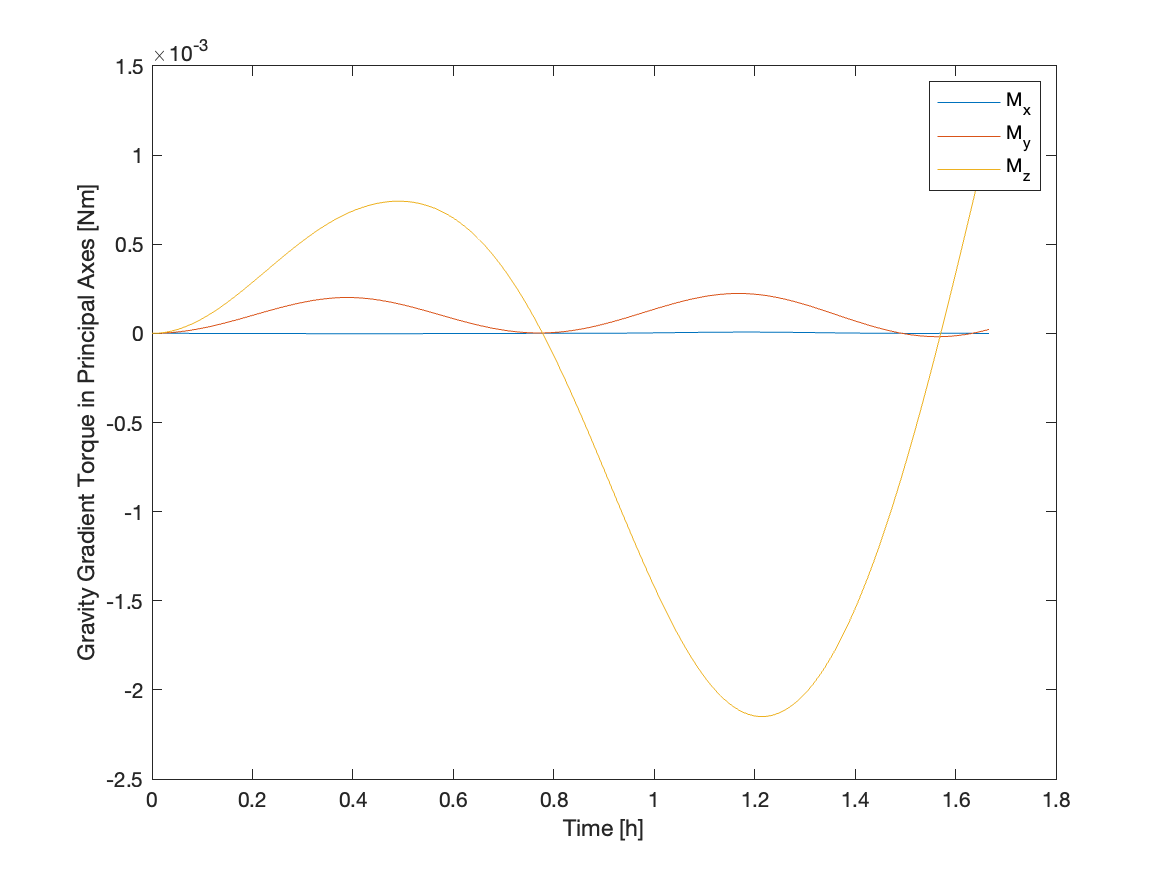
\includegraphics[scale=0.6]{Images/ps5_problem3_grav.png}
\caption{Numerical simulation of gravity gradient torques}
\label{fig:ps5_problem3_grav}
\end{figure}

\begin{figure}[H]
\centering
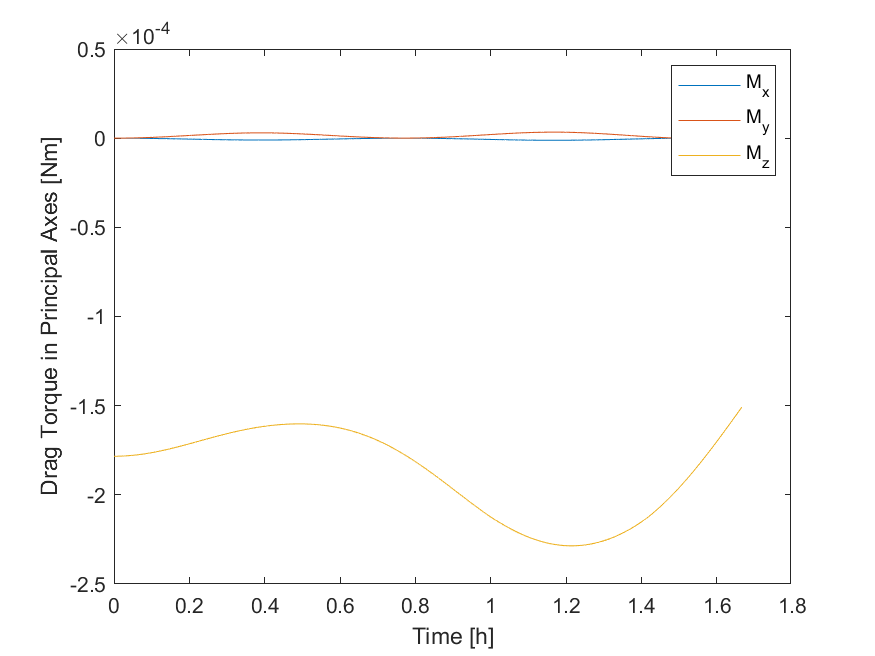
\includegraphics[scale=0.6]{Images/ps5_problem3_drag.png}
\caption{Numerical simulation of drag torques}
\label{fig:ps5_problem3_drag}
\end{figure}

\begin{figure}[H]
\centering
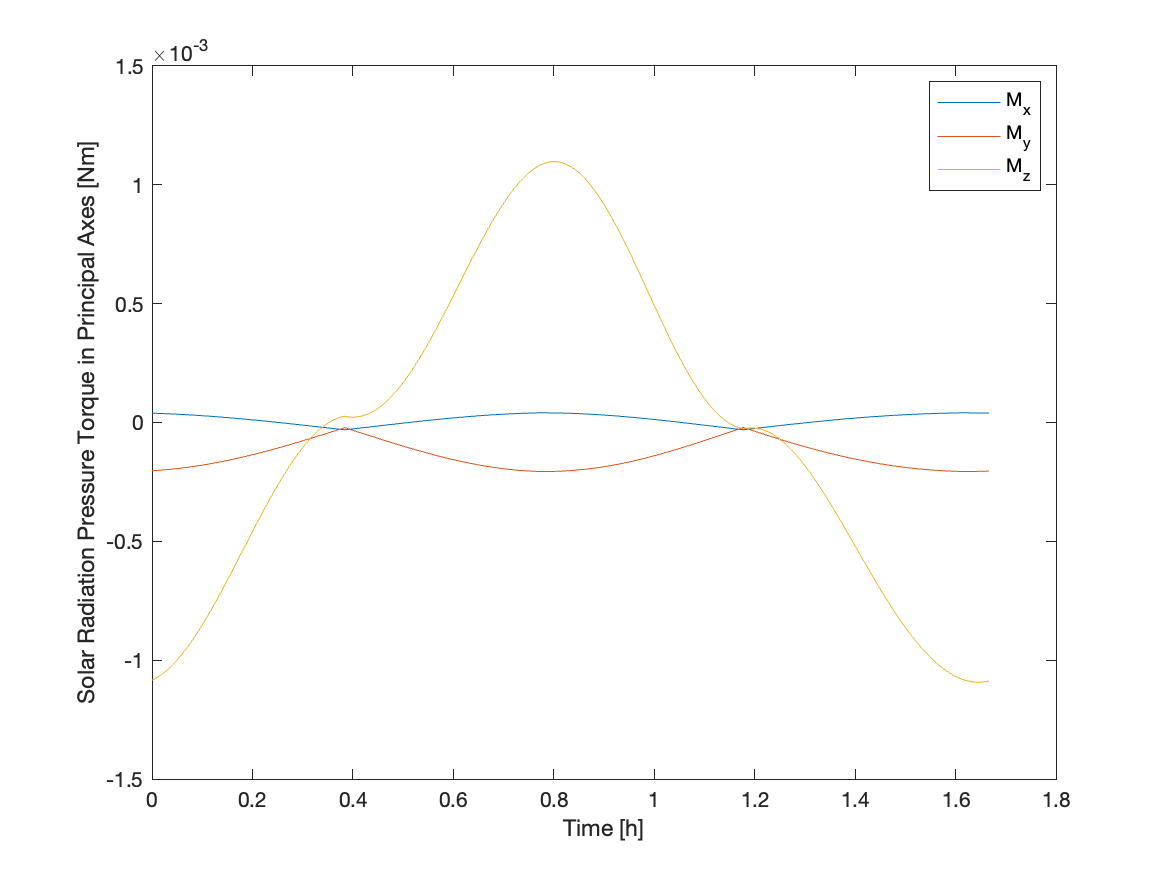
\includegraphics[scale=0.6]{Images/ps5_problem3_srp.png}
\caption{Numerical simulation of solar radiation pressure torques}
\label{fig:ps5_problem3_srp}
\end{figure}

\begin{figure}[H]
\centering
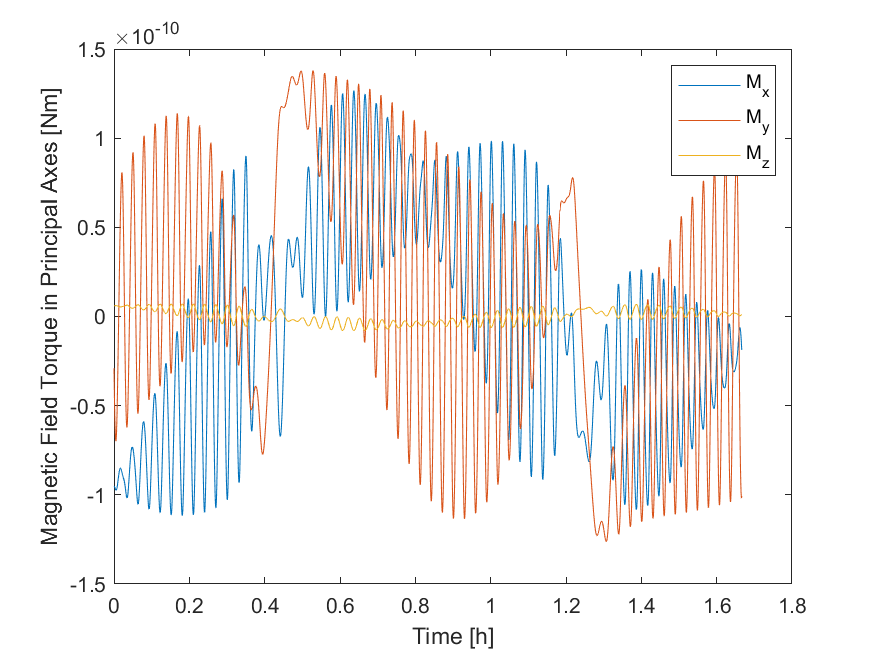
\includegraphics[scale=0.6]{Images/ps5_problem3_mag.png}
\caption{Numerical simulation of magnetic field torques}
\label{fig:ps5_problem3_mag}
\end{figure}

%%%%%%%%%%%%%%%%%%%%%%%%%%%%%%%%%%%%%%%%%%%%%%%%%%%%%%%%%%%%%%%%%%%%%%%%%%%%%%%%%%%%%%%%%%%%%%%%%%%%%%%%%%%%%%%%%%%%%%%%%%%%%%%%%%%%%%%%%%%%%%%%%%%%%%%%%%%%%%%%%%%%%%%%%%%%%%%%%%%%%%%%%%%%%%%%%%%%%%%%%%%%%%%%%%%%%%%%%%% 
% \section{\Large CONCLUSION}

\newpage
\section{\Large REFERENCES}
\printbibliography[heading=none]

\appendix

\section{APPENDIX A: CODE}
The following MATLAB code are used in the original AA 279C problem sets. The full code (including Simulink models) and resource files can be found in the GitHub repository: \url{https://github.com/zhao-harry/aa-279c-project}

\subsection{Problem Set 1 – Mass and Surface Properties}
\lstinputlisting{src/ps1.m}

\newpage
\subsection{Problem Set 2 – Dynamics}
\lstinputlisting{src/ps2.m}
\lstinputlisting{src/plotECI.m}
\lstinputlisting{src/eulerPropagator.m}
\lstinputlisting{src/ellipsoidEnergy.m}
\lstinputlisting{src/ellipsoidMomentum.m}
\lstinputlisting{src/polhode.m}
\lstinputlisting{src/polhode2D.m}

\newpage
\subsection{Problem Set 3 – Axial-Symmetric and Kinematics}
\lstinputlisting{src/ps3.m}
\lstinputlisting{src/plotTriad.m}

\newpage
\subsection{Problem Set 4 – Equilibrium and Gravity Gradient}
\lstinputlisting{src/ps4.m}
\lstinputlisting{src/kinEulerAngleWheel.m}

\newpage
\subsection{Problem Set 5 – Gravity Gradient Stability and Perturbations}
\lstinputlisting{src/ps5.m}
\lstinputlisting{src/plotGravGradStability.m}
\lstinputlisting{src/orbitTorque.m}
\lstinputlisting{src/drag.m}
\lstinputlisting{src/srp.m}
\newpage
\textbf{The following set of functions are used for our fourth-order magnetic field model.}
\lstinputlisting{src/magFieldTorque.m}
\lstinputlisting{src/magFieldEarth.m}
\lstinputlisting{src/getdPdTheta.m}
\lstinputlisting{src/getKnm.m}
\lstinputlisting{src/getPnm.m}

\newpage
\subsection{Problem Set 6 – Attitude Determination}
\lstinputlisting{src/ps6.m}
\lstinputlisting{src/DAD2Vec.m}
\lstinputlisting{src/DAD.m}
\lstinputlisting{src/qMethod.m}
\lstinputlisting{src/kinEulerStepRK4.m}

\newpage
\subsection{Problem Set 7 – MEKF Time Update}
\lstinputlisting{src/ps7.m}

\newpage
\subsection{Problem Set 8 – MEKF Measurement Update}
\lstinputlisting{src/ps8.m}
\lstinputlisting{src/starTracker.m}
\lstinputlisting{src/sunSensor.m}

\newpage
\subsection{Problem Set 9 – Control}
\lstinputlisting{src/ps9.m}

\newpage
\subsection{Problem Set 10 – Final Project}
\lstinputlisting{src/ps10.m}

\end{document}